\documentclass[12pt, a4paper]{article}

\usepackage[utf8x]{inputenc}
\usepackage[german]{babel}
\usepackage{enumitem}
\usepackage{anyfontsize}
\usepackage{listings}
\usepackage{color}
\usepackage{graphicx}
\usepackage{float}
\usepackage[babel,german=quotes]{csquotes}

% Anpassungen für Programm-Codes
\renewcommand{\lstlistingname}{Programm-Code} 
\lstset{
	extendedchars=\true,
	inputencoding=utf8x,
	belowcaptionskip=1\baselineskip,
	breaklines=true,
	frame=L,
	xleftmargin=\parindent,
	showstringspaces=false,
	basicstyle=\footnotesize\ttfamily
}
\lstdefinestyle{customPHP}{
	language=PHP,
	keywordstyle=\bfseries\color{green},
	commentstyle=\itshape\color{red},
	identifierstyle=\color{blue},
	stringstyle=\color{cyan},
}
\lstdefinestyle{customHTML}{
	language=PHP,
	keywordstyle=\bfseries\color{green},
	commentstyle=\itshape\color{red},
	identifierstyle=\color{blue},
	stringstyle=\color{cyan},
}

\title{Anleitung für Administratoren\\
SIS - School Information Service}

\author{Florian \textsc{Buchberger}\\Marco \textsc{Handle}\\Matthias \textsc{Klotz}\\Mathias \textsc{Weiland}}
\date{\today}

\usepackage{color}

\usepackage[T1]{fontenc}
\usepackage{titlesec, blindtext, color}

\definecolor{gray75}{gray}{0.75}
\newcommand{\hsp}{\hspace{20pt}}
\titleformat{\section}[hang]{\Huge\bfseries}{\thesection\hsp\textcolor{gray75}{||}\hsp}{0pt}{\Huge\bfseries}

%\setcounter{secnumdepth}{4}
%\setcounter{tocdepth}{3}

\begin{document}

\maketitle

\newpage

\tableofcontents

\newpage

\section{Einleitung}

Dies ist die Anleitung für den Abteilungsvorstand bzw. Super User für das School Information Service der HTL Anichstraße. Diese Anleitung wurde im Zuge der Diplomarbeit vom SIS-Team geschrieben, um alle Funktionen unseres Systems zu dokumentieren

\newpage
\section{News}

Um die News zu bearbeiten, klicken Sie im \enquote{Data-Input-Menu} auf den Punkt \enquote{News hinzufügen}
\\
Nach dem Öffnen der Seite werden die eingetragenen News angezeigt.
\\

\subsection{News bearbeiten/hinzufügen}
\begin{description} 
\item[Titel] Titel der angezeigt werden soll.
\item[Text] Text der angezeigt werden soll.
\item[Abt.] Abteilung für welche die News angezeigt werden soll. Wenn dieses Feld leer ist, wird die News in allen Abteilungen angezeigt.
\item[Anzeigebeginn-Datum] Datum ab welchem die News angezeigt werden soll.
\item[Anzeigeend-Datum] Datum bis zu welchem die News angezeigt werden soll.
\item[Anzeigen] Zeigt an ob die News angezeigt wird. Wenn ein Newsbeauftragter eine News hinzufügt, ist dieser Punkt nicht gewählt und muss vom Abteilungsvorstand ausgewählt werden, um die News freizugeben. 
\item[Ersteller] In dieses Feld kann nichts eingegeben werden. Es dient dazu, dass der Abteilungsleiter weiß, wer die News erstellt hat.
\item[Nur Website] Wenn dieser Punkt ausgewählt ist,wird die News nur auf der Website oder in der App angezeigt und nicht auf den Monitoren.
\end{description}

\subsection{News löschen}

\newpage
\section{Monitore}

Um in die Einstellungen für die Monitore zu gelangen, klicken Sie im \enquote{Data-Input-Menü} auf den Punkt \enquote{Monitore verwalten} (siehe \autoref{fig:instr_admin_monitors_dimenu}).\\
\\
\begin{figure}[H]
\centering
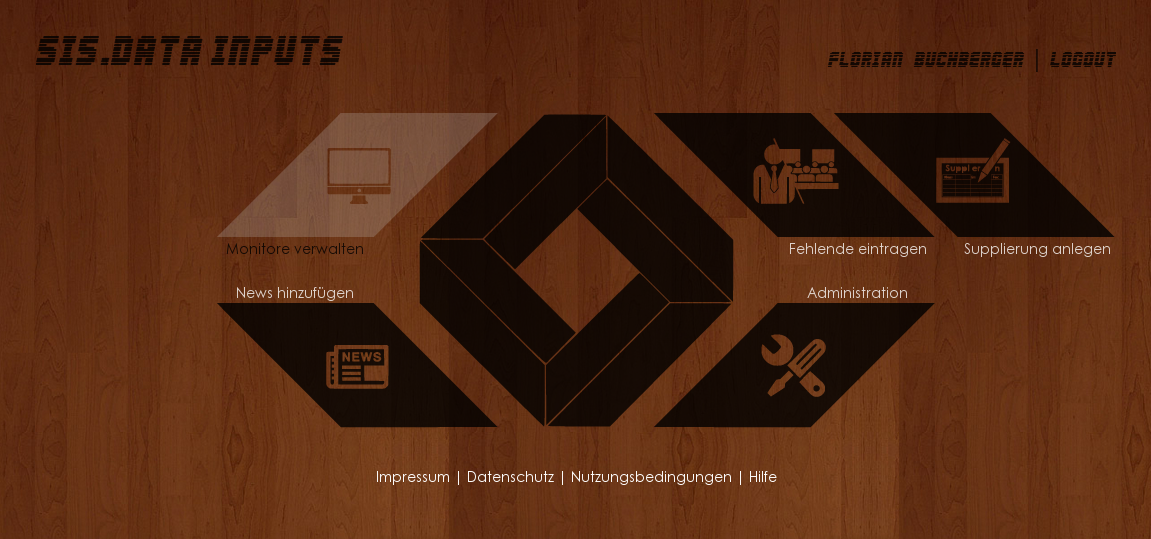
\includegraphics[keepaspectratio=true, width=14cm]{images/screenshots/data-inputs.png}
\caption{Data-Input-Menü}
\label{fig:instr_admin_monitors_dimenu}
\end{figure}
Nach dem Öffnen der Seite werden oben im Fenster die aktiven Monitore aufgelistet. Darunter sind die Einstellungen zu finden.\\
\\
\begin{figure}[H]
\centering
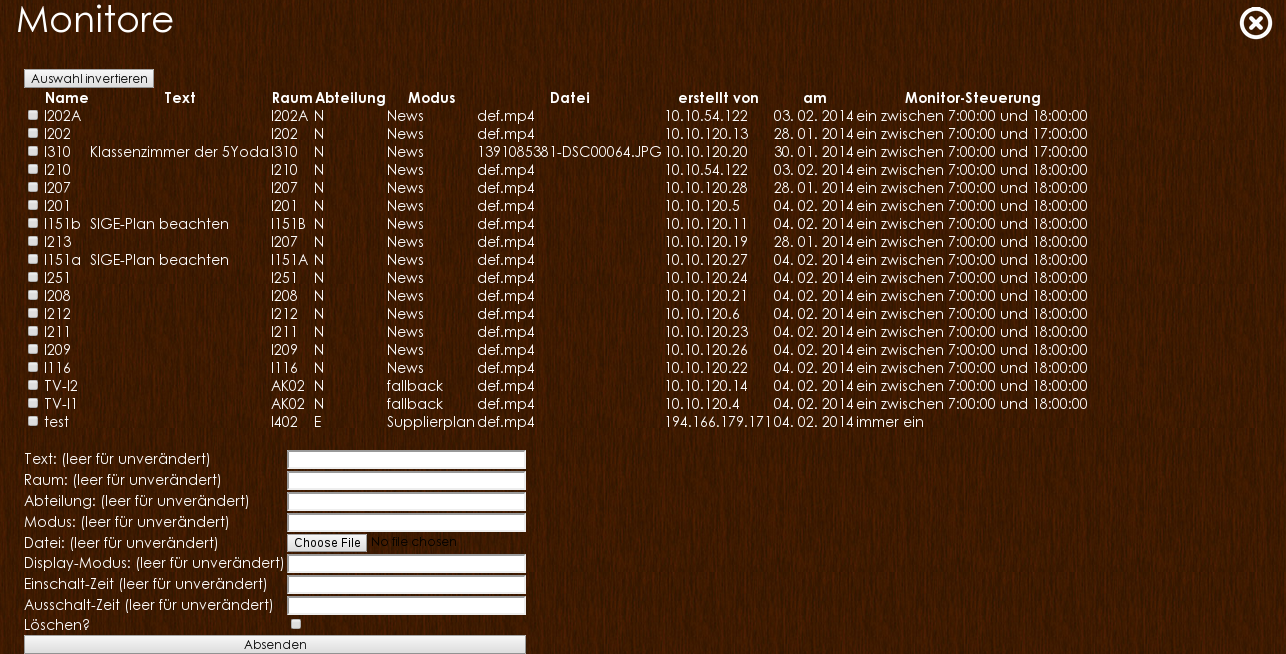
\includegraphics[keepaspectratio=true, width=14cm]{images/screenshots/monitors.png}
\caption{Monitor-Einstellungen}
\label{fig:instr_admin_monitors_site}
\end{figure}
Die Monitore, deren Einstellungen verändert werden sollen, müssen mit einem Klick auf die Checkbox links neben der Anzeige ausgwählt werden. Es können mehrere ausgewählt werden. Mit dem Button \enquote{Auswahl invertieren} werden alle gesetzten Checkbox rückgesetzt, und umgekehrt.
\\
\subsection{Hinzufügen}

\subsubsection{Software}
\label{sec:instr_monitor_software}
Für folgendes wird vorausgesetzt, dass das von uns zur Verfügung gestellte Image verwendet wird. Dieses kann unter folgender Adresse runtergeladen werden:\\ \href{https://sis.htlinn.ac.at/sis.img}{https://sis.htlinn.ac.at/sis.img}\\
Das Image ist 4 GB groß, wir empfehlen deshalb, das Image ohne Proxy-Einstellung mit der Adresse \href{http://sis.clients.htlinn.ac.at/sis.img}{http://sis.clients.htlinn.ac.at/sis.img} im Schulnetz zu laden. Das Image sollte auf eine SD-Karte mit mindestens 3965190144 Bytes Speicherplatz gespielt werden (Getestet wurde mit \enquote{SanDisk Extreme 4GB}).\\
Der vordefinierte Benutzer hat die Kennung \enquote{pi} und das Passwort \enquote{sis}.\\
\\
Ein neuer Monitor kann nicht über das Web-Interface hinzugefügt werden, die Monitore registrieren sich selbstständig am Server. Nach der Registrierung stehen sie zur Verwaltung zur Verfügung.\\
Damit sich die Monitore registrieren können, müssen sie ihre eigene Identität kennen. Diese wird in der Datei /etc/sis.conf definiert.\\

\begin{lstlisting}[style=custom,  caption={Beispiel /etc/sis.conf},label={lst:instr_admin_sisconf}]
name=test-monitor
\end{lstlisting}
Die Form des Namenseintrags ist im Beispiel  \autoref{lst:instr_admin_sisconf} ersichtlich.\\
Wenn der Name des Monitors geändert wird, sollte aus Gründen der Übersichtlichkeit und Nachvollziehbarkeit darauf geachtet werden, dass der Hostname des Raspberry Pis mit dem Namen übereinstimmt. Dazu wird die Datei /etc/hostname bearbeitet. Damit der Host nicht neu gestartet werden muss, kann mit dem Befehl \enquote{hostname} der Hostname zusätzlich auch direkt geändert werden. \\
\textit{Beispiel}: hostname I386\\
\\
\textit{Achtung:} Da es zu Problemen mit manchen Programmen (wie zum Beispiel \textit{sudo}) kommen kann, sollte in er Datei /etc/hosts ein Eintrag für den Hostnamen angelegt werden, welcher auf die lokale Adresse zeigt (üblicherweise die Loopback-Adresse 127.0.1.1).\\
\\
\textit{Achtung:} Die Software lässt es zu, dass mehrere Monitore den selben Namen tragen. Dies sollte allerdings vermieden werden.

\subsubsection{Hardware}
Die Header Platine für den Raspberry Pi wird auf demselben aufgesteckt (siehe \autoref{fig:report_hardware_Headergesteckt}). Der Monitor wird über HDMI mit dem Raspberry verbunden, die Stromversorgung ist, wie beim Raspberry üblich, mit einem USB-zu-microUSB-Adapter und einem dementsprechenden Netzteil herzustellen.\\
Als Netzwerkanbindung kann entweder die LAN-Buchse oder ein W-LAN-Stick verwendet werden. Hierbei ist zu beachten, dass der Computer, sofern er mit der unter  \autoref{sec:instr_monitor_software} beschriebenen Software betrieben wird, keine statische IP-Adresse eingetragen hat, es ist daher ein DHCP-Server notwendig. Bei Verwendung von W-LAN ist zusätzlich zu beachten, dass der Raspberry von sich aus das W-LAN \enquote{HTL-SIS} mit dem passenden WPA2-Pre-Shared-Key eingetragen hat, bei einer Änderung muss dieser angepasst werden.\\
\\
Die Verbindung zwischen dem Raspberry und der modifizierten Steckdose (siehe FTKL-Bericht) wird mit einem ausgekreuzten Mono-Klinke-Kabel hergestellt.\\
\textit{Beachte:} Wenn der Computer an die modifizierte Steckdose angeschlossen wird, dann kann er sich logischerweise nicht selbst einschalten, deshalb sollte nur der entsprechende Monitor daran angeschlossen werden.\\
\\
Sollte sich nach dem ersten Start des Computers der Monitor nicht nach spätestens 5 Minuten selbstständig einschalten, so kann es sein, dass die nicht vorhandene HDMI-Daten-Sinke den Start blockiert. In diesem Fall sollte der Monitor während dem Starten auf eine normale Steckdose gesteckt werden, läuft in dem Fall der Raspberry, so sollte die Steckdose, die Platine, sowie die Kabel überprüft und gegebenenfalls getauscht werden.

\begin{figure}[H]
\centering
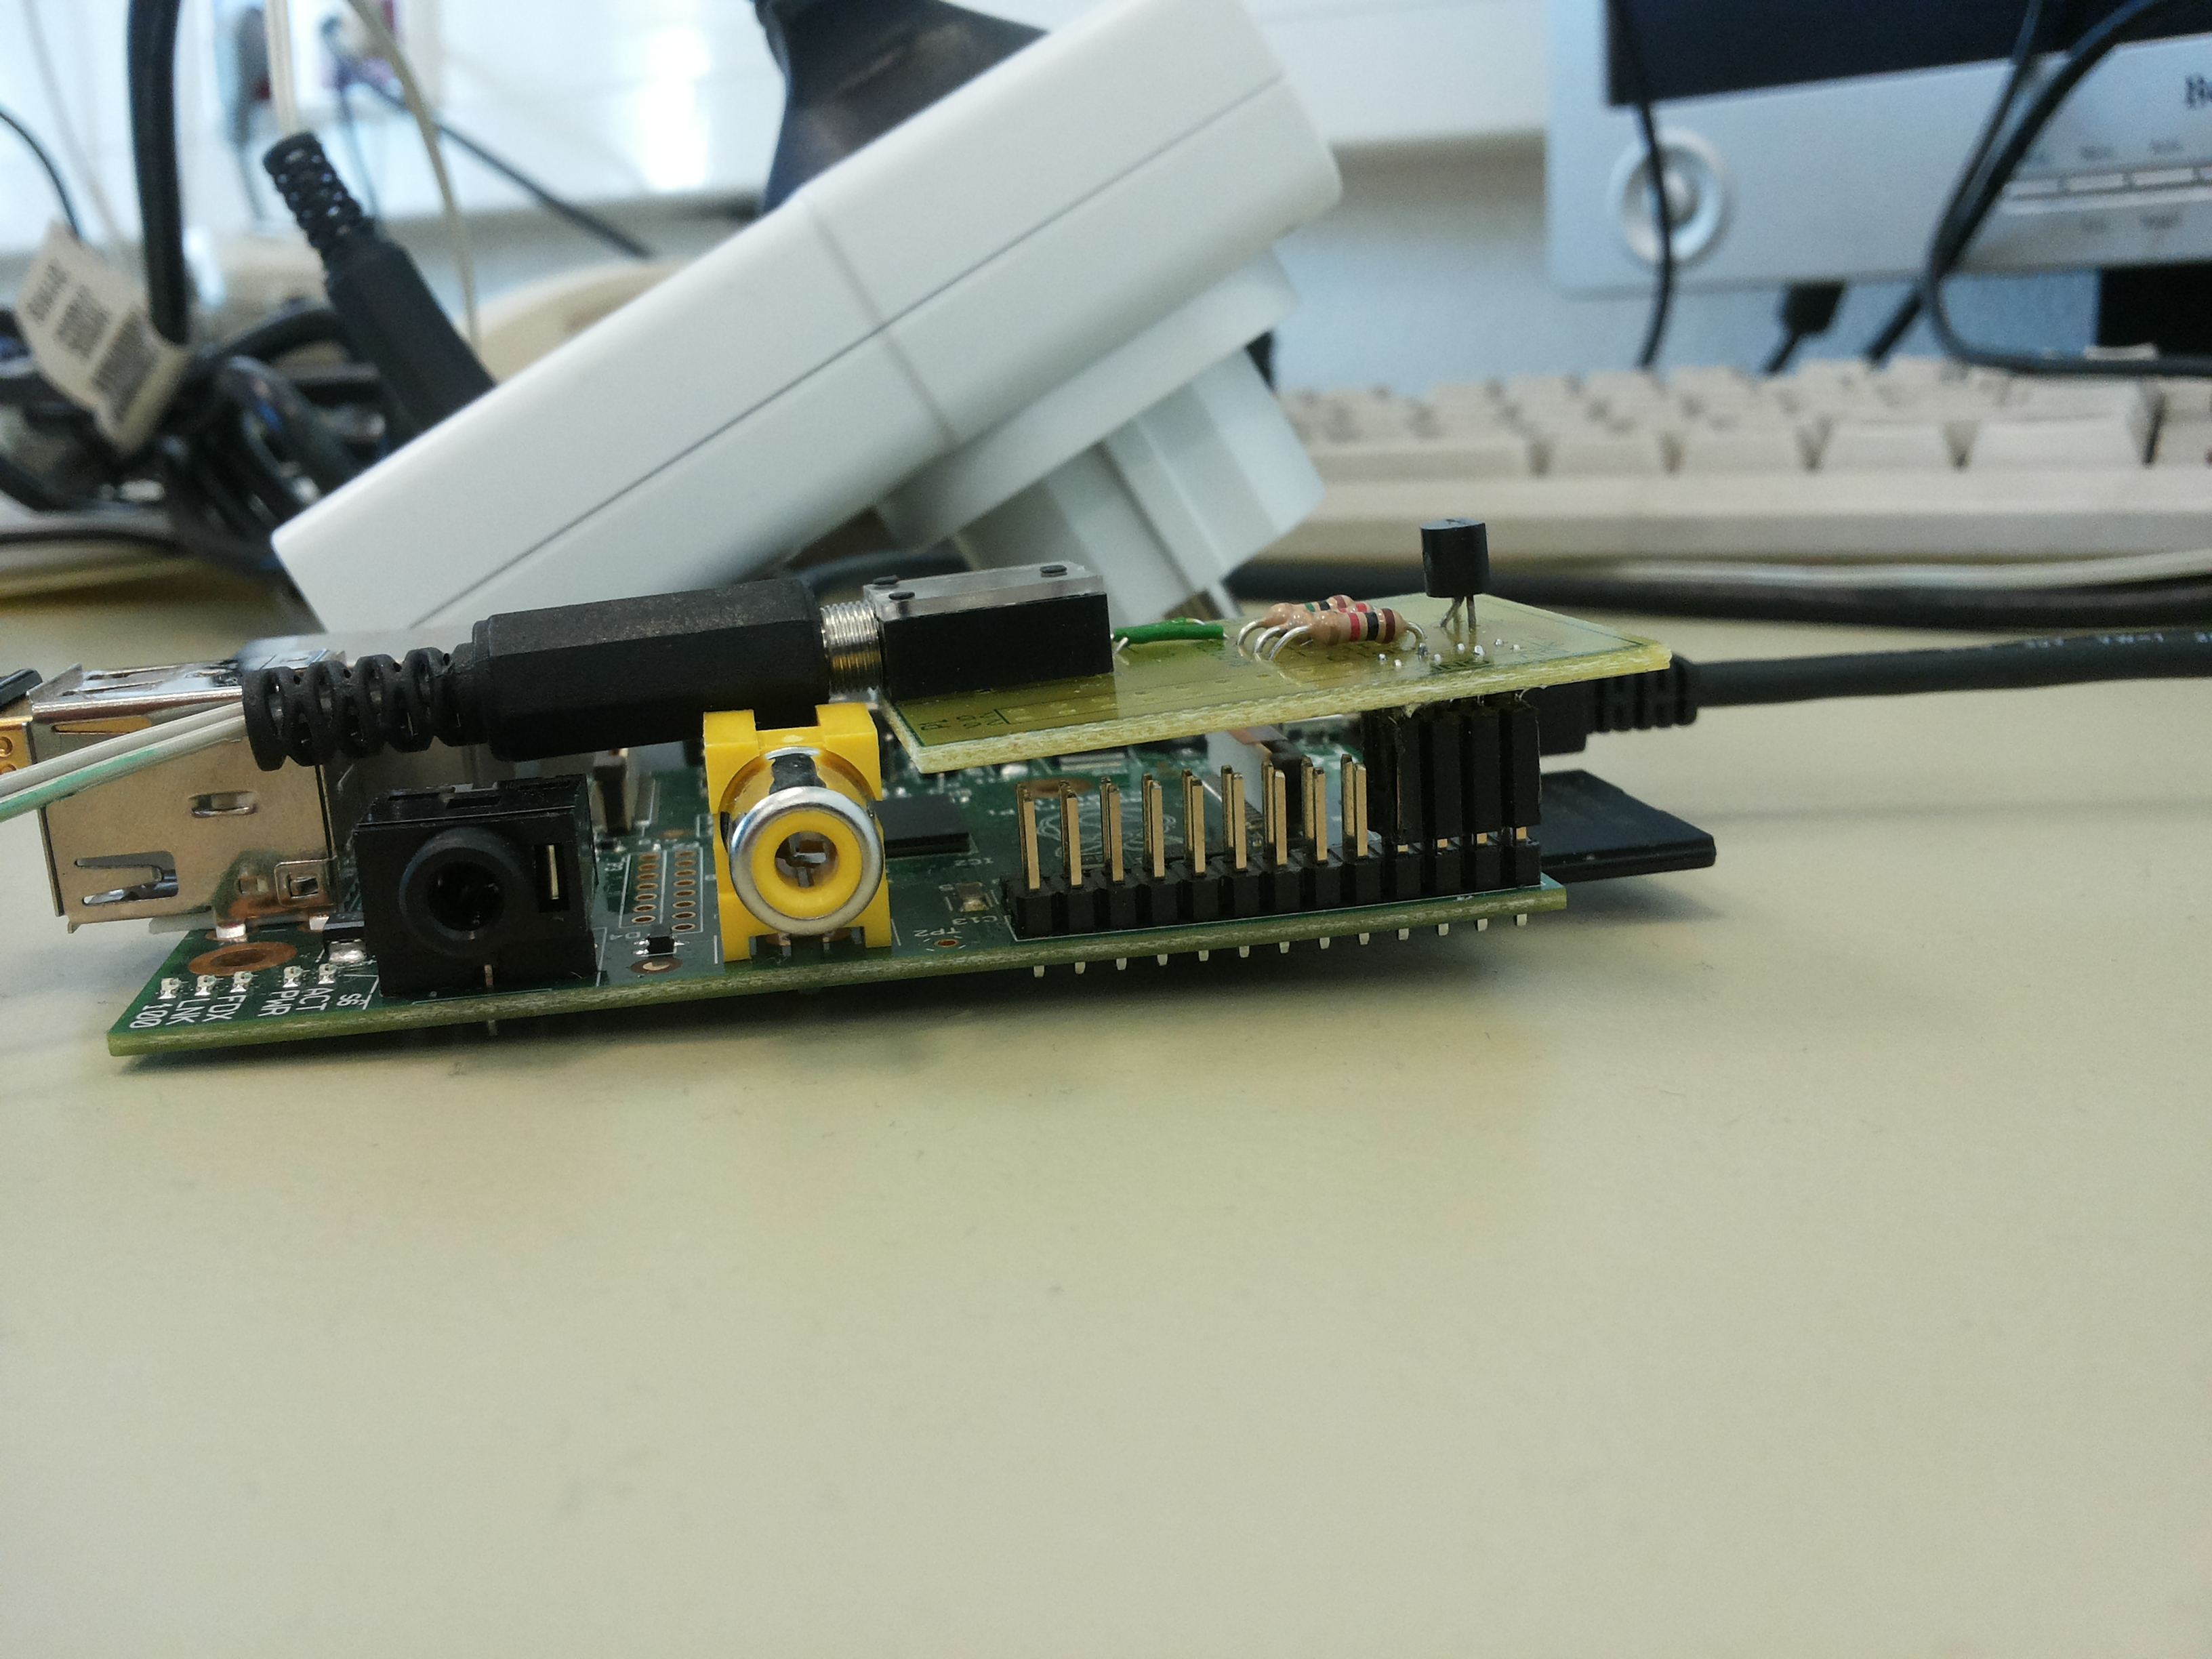
\includegraphics[keepaspectratio=true, width=10cm]{images/rpi/rpi_header_gesteckt.jpg}
\caption{Aufbau Header}
\label{fig:report_hardware_Headergesteckt}
\end{figure}

\begin{figure}[H]
\centering
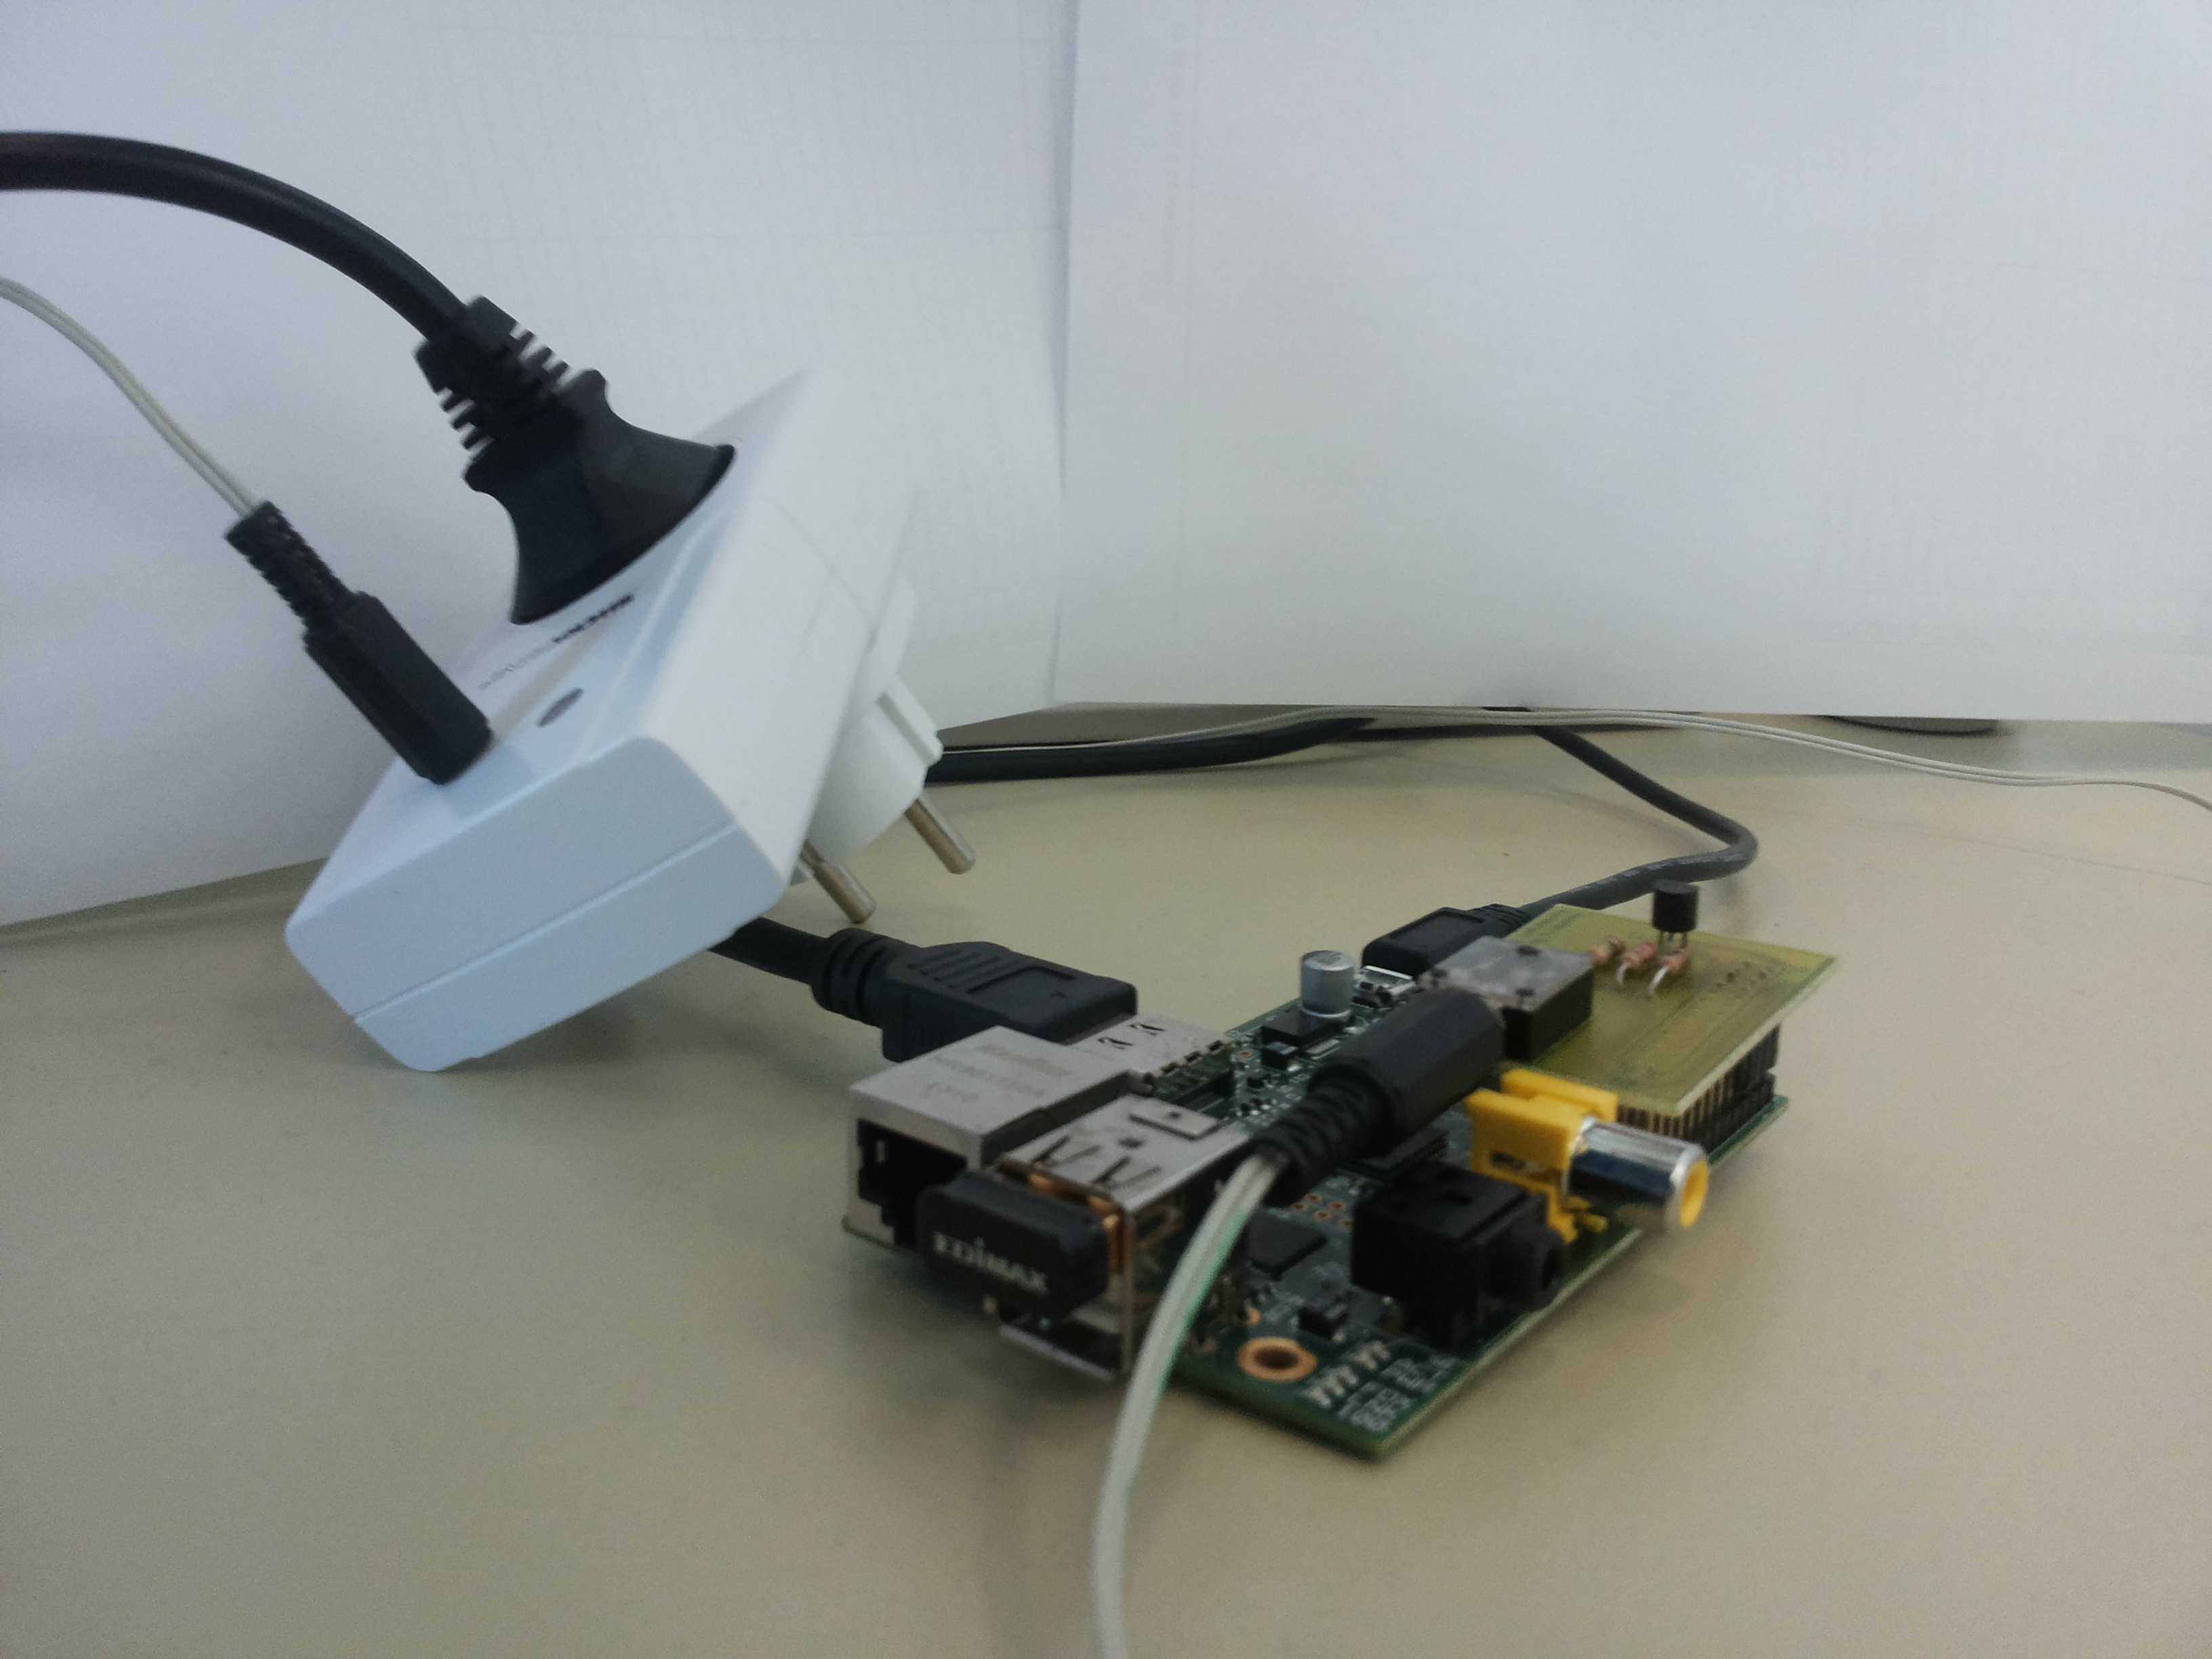
\includegraphics[keepaspectratio=true, width=10cm]{images/rpi/rpi_gesamt.jpg}
\caption{Gesamtaufbau}
\label{fig:report_hardware_Gesamt}
\end{figure}

\subsection{Entfernen}

Um einen Monitor aus der Liste der aktiven Monitore zu entfernen, wählen Sie den jeweiligen Monitor über die Checkbox aus, setzen Sie die \enquote{Löschen?}-Checkbox und klicken Sie auf \enquote{Änderungen anwenden}.\\
\\
\textit{Achtung:} Sollte der Monitor nach dem Entfernen noch eingeschalten sein, so wird sich dieser, sofern die Standard-Konfiguration eingestellt ist, wieder neu registrieren.

\subsection{Text verändern}

Der Text, der am linken unterem Eck des Monitors kann über das Eingabefeld \enquote{Text} geändert werden. Wird das Feld leer gelassen, so wird der alte Wert beibehalten.\\
\\
\textit{Achtung:} Leerzeichen werden nicht als leer erkannt.

\subsection{Raum verändern}

Für die Darstellung des Stundenplanes des jeweiligen Raumes wird jedem Monitor ein Raum zugeordnet. Diese Einstellung kann über das Eingabefeld \enquote{Raum} angepasst werden. Durch Doppelklick auf das Eingabefeld öffnet sich - sofern der verwendete Browser diese Funktion unterstützt - ein Menü, in dem durch Eingeben gesucht werden kann. Wird das Feld leer gelassen, so wird der alte Wert beibehalten.

\subsection{Abteilung verändern}

Die News können Abteilungen zugeordnet werden. Ebenso ist der Supplierplan für jede Abteilung anders. Als Folge daraus gibt es eine Einstellungsmöglichkeit für die Abteilung. Durch Doppelklick auf das Eingabefeld öffnet sich - sofern der verwendete Browser diese Funktion unterstützt - ein Menü, in dem durch Eingeben gesucht werden kann. Wird das Feld leer gelasen, so wird der alte Wert beibehalten.

\subsection{Modus verändern}

Um die ausgewählten Monitore auf Supplierplan, Stundenplan, News etc. umzuschalten, wird das Eingabefeld \enquote{Modus} verwendet. In diesem Feld sind folgende Werte zulässig:
\begin{itemize}
	\item News
	\item Stundenplan
	\item Supplierplan
	\item Supplierplan \& News
	\item Bild
	\item (Video)
	%\item (fallback)
\end{itemize}
Durch Doppelklick auf das Eingabefeld öffnet sich - sofern der verwendete Browser diese Funktion unterstützt - ein Menü mit den möglichen Werten. Wird das Feld leer gelassen, so wird der alte Wert beibehalten.\\
\\
Der Modus \enquote{Video} ist zwar implementiert, allerdings ist der Raspberry Pi nicht in der Lage, die Videos wiederzugeben.\\
%Der Modus \enquote{fallback} fährt den Monitor auf das FTKL-Schnitzel-Suppla-Projekt.\\ 
%\textit{Achtung:} Es ist nicht über das Web-Interface möglich, den Monitor wieder auf das SIS-Projekt zurückzuholen.

\subsection{Datei verändern}

Für die Modi \enquote{Bild} und \enquote{Video} muss eine Datei hochgeladen werden, welche dann angezeigt wird.\\ 
Unterstützte Dateitypen sind:
\begin{itemize}
	\item JPG, JPEG
	\item PNG
	\item GIF
	\item MP4, MPEG
\end{itemize}
Die maximale Dateigröße ist limitiert durch:
\begin{itemize}
	\item das Upload-Script auf 800 MB
	\item den Upload-HTML-Tag auf 800 MB
	\item die PHP-Konfiguration am Server (Stand: 2014-02-28) auf 128 MB
\end{itemize}
Wird das Feld leer gelassen, so wird der alte Wert beibehalten.\\

\subsection{Display-Modus verändern}

Die Raspberry Pis verfügen über einen Mechanismus, um den angeschlossenen Monitor ein- bzw auszuschalten.\\
Es sind folgende Modi möglich:
\begin{itemize}
	\item permanent Ein
	\item permanent Aus
	\item automatisch
\end{itemize}
Im automatischen Modus werden die Einstellungen von \ref{instr_admin_moni_time_on} und \ref{instr_admin_moni_time_off} verwendet.\\
\\
Wird das Feld leer gelassen, so wird der alte Wert beibehalten.\\

\subsubsection{Einschalt-Zeit}
\label{instr_admin_moni_time_on}

Bestimmt die Zeit, an dem sich der angeschlossene Monitor einschalten soll.\\
\textit{Beispiele:}
\begin{tabbing}
\hspace{2cm}\=\kill
7 \> 7 Uhr früh\\ 
6:35 \> 6:35 früh\\
17:05:11 \> 5:05:11 nachmittags
\end{tabbing}
Wird das Feld leer gelassen, so wird der alte Wert beibehalten.\\

\subsubsection{Ausschalt-Zeit}
\label{instr_admin_moni_time_off}

Analog zu \ref{instr_admin_moni_time_on}.


\newpage
\section{Fehlende}\label{sec:instr_admin_absentees}

Im Menü \enquote{Data-Input} (siehe \autoref{fig:instr_admin_absentees_dimenu}) können über den Auswahlpunkt \enquote{Fehlende eintragen}  fehlende Lehrer und fehlende Klassen eingegeben werden. Es öffnet sich ein weiteres Menü (siehe \autoref{fig:instr_admin_absentees_menu}) mit der Wahlmöglichkeit zwischen Lehrer und Klassen.
\begin{figure}[H]
\centering
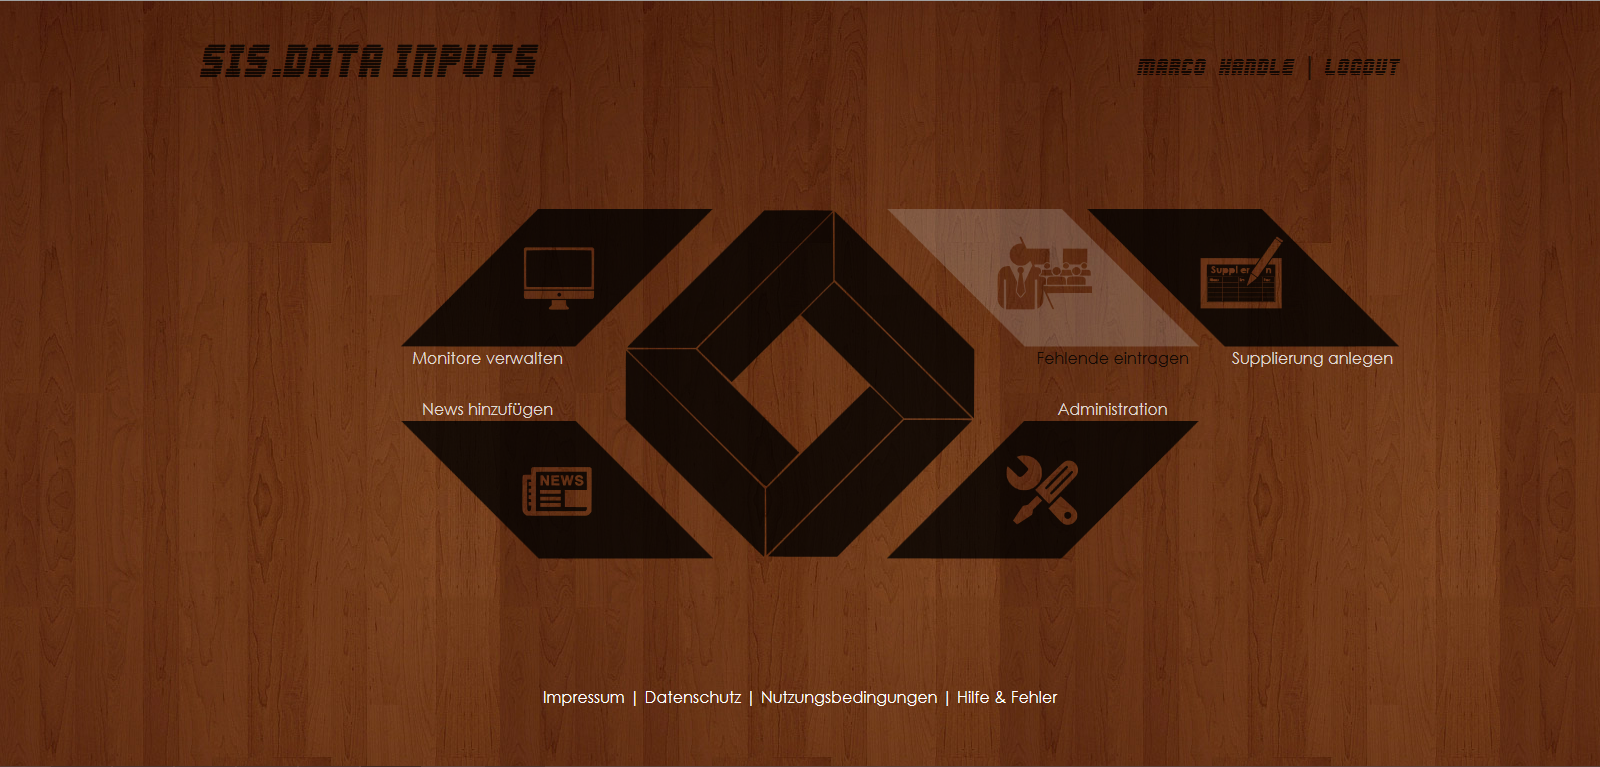
\includegraphics[keepaspectratio=true, width=14cm]{images/screenshots/data-inputs2.png}
\caption{Data-Input-Menü}
\label{fig:instr_admin_absentees_dimenu}
\end{figure}
\begin{figure}[H]
\centering
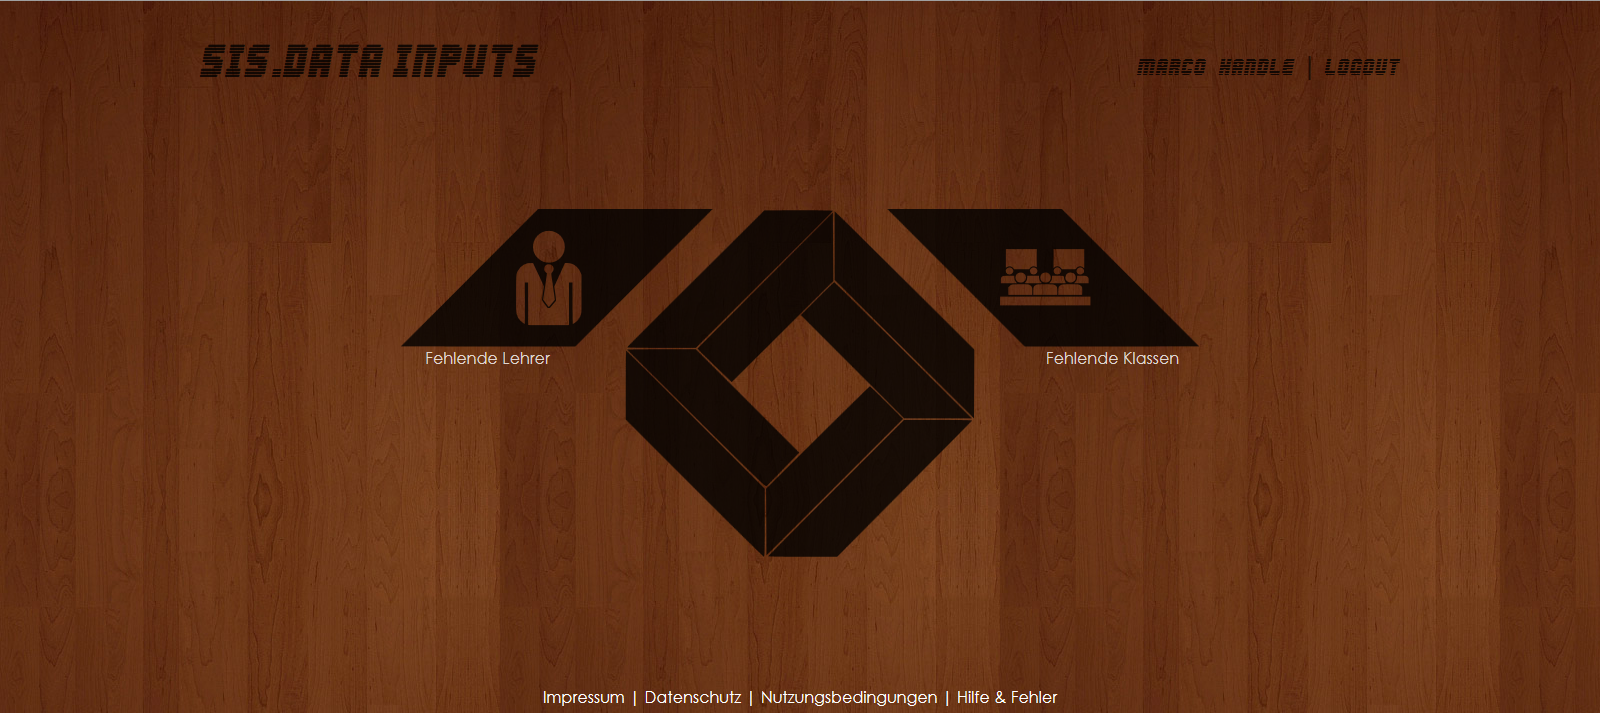
\includegraphics[keepaspectratio=true, width=14cm]{images/screenshots/data-inputs_absentees.png}
\caption{Fehlende Auswahl}
\label{fig:instr_admin_absentees_menu}
\end{figure}
\subsection{Fehlende Lehrer}
\label{sec:instr_admin_absentees_teacher}
In der tabellarischen Eingabemaske (siehe \autoref{fig:instr_admin_absentees_Lehrer}) können nun fehlende Lehrer hinzugefügt, Einträge geändert oder gelöscht werden. Standardmäßig werden beim Öffnen der Eingabemaske die für den aktuellen Tag erfassten Fehlenden Lehrer angezeigt.
\subsubsection{Fehlenden Lehrer Hinzufügen} \label{sec:instr_admin_absentees_teacher_insert}
Als erster Schritt ist das Datum des Tages auszuwählen, für den fehlende Lehrer erfasst werden. Dies kann entweder durch das Vor- und Zurückblättern mit den Pfeiltasten erfolgen oder durch eine manuelle Eingabe (Format yyyy-mm-dd). Die manuelle Eingabe ist mit der Enter-Taste zu bestätigen. Dieses Datum wird in neuen Eingabezeilen automatisch in das Feld Starttag eingetragen. Dann sind die einzelnen Eingabefelder zu befüllen.\\
\begin{table}
\centering
\begin{tabular}{p{3 cm}p{6 cm}p{5 cm}}
   \toprule
   \textbf{Eingabefeld} & \textbf{Typ} & \textbf{Wertebereich} \\
   \midrule
          \textbf{Lehrer} & Text \newline Kürzel des Lehrers -Auswahl aus Listenfeld & \\
          \hline
          \textbf{Starttag} & Datum \newline Wird automatisch eingetragen und kann nicht verändert werden &  \\
          \hline
          \textbf{Start-Stunde} & nummerisch & 1-16\\
          \hline
          \textbf{Endtag} & Datum \newline Standardmäßig wie Starttag ist auf gewünschtes Datum zu ändern & Größer oder gleich Starttag und kein Samstag oder Sonntag \\
          \hline
          \textbf{End-Stunde} & nummerisch & 1-16 \newline Wenn Starttag und Endtag gleich, dann größer als Start-Stunde\\
          \hline
          Grund & Text - optional \newline Freie Texteingabe für den Grund des Fehlens & \\
   \bottomrule
\end{tabular}
\caption{Eingabefelder Fehlende}
\end{table}
Sind alle Pflicht-Eingabefelder befüllt, wird durch Drücken auf Übernehmen die Eingabezeile übernommen, wobei vorher eine Plausibilitätsüberprüfung vorgenommen wird. Sollte eine Fehleingabe bemerkt werden, wird in einem Popup-Fenster (siehe \autoref{fig:instr_admin_absentees_fail}) das fehlerhafte Feld angezeigt. Die Eingabefelder werden gelöscht und müssen neu erfasst werden. Bei einer fehlerfreien Übernahme wird in der Eingabezeile die Checkbox Löschen und eine weitere Eingabezeile angezeigt.
\subsubsection{Eingabezeile verändern}
Ein bereits übernommener Eintrag kann noch nachträglich verändert werden. Die Änderungen sind in den Feldern vorzunehmen und dann wie unter \autoref{sec:instr_admin_absentees_teacher_insert} für jede Eingabezeile zu übernehmen.
\subsubsection{Eingabezeile löschen}
Das Löschen eines fehlenden Lehrers erfolgt über die Checkbox \enquote{Löschen} der entsprechenden Eingabezeile. Diese muss ausgewählt werden und dann mit Übernehmen bestätigt werden. Es erfolgt keine weitere Sicherheitsabfrage und der Eintrag ist \textbf{unwiderruflich} gelöscht (siehe \autoref{fig:instr_admin_absentees_Leherer_delete}).
\begin{figure}[H]
\centering
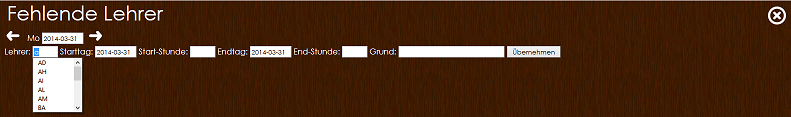
\includegraphics[keepaspectratio=true, width=16cm]{images/screenshots/absentees_teacher.png}
\caption{Fehlende Lehrer}
\label{fig:instr_admin_absentees_Lehrer}
\end{figure}
\begin{figure}[H]
\centering
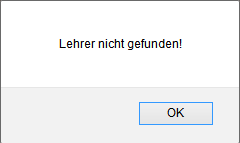
\includegraphics[keepaspectratio=true, width=4cm]{images/screenshots/input_fail_teacher.png}
\caption{Falsche Eingabe}
\label{fig:instr_admin_absentees_fail}
\end{figure}
\begin{figure}[H]
\centering
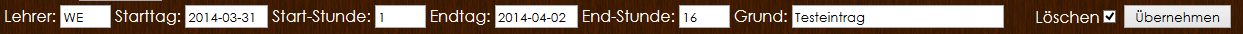
\includegraphics[keepaspectratio=true, width=16cm]{images/screenshots/absentees_teacher_delete.png}
\caption{Fehlenden Lehrer löschen}
\label{fig:instr_admin_absentees_Leherer_delete}
\end{figure}
\subsection{Fehlende Klassen}
Die Erfassung von Fehlenden Klassen erfolgt analog jener der Fehlenden Lehrer. Die Eingabemenüs und Eingabefelder sind sinngemäß wie unter \autoref{sec:instr_admin_absentees_teacher} beschrieben zu verwenden.

\newpage
\section{Supplierungen}

Das Erfassen von Supplierungen kann im Menü \enquote{Data Input} gestartet werden (siehe \autoref{fig:instr_substitudes_dataInput}). Es wird die Eingabemaske für die Abteilung des Users geöffnet (siehe \autoref{fig:instr_substitudes_subNoFree}). Der Super-User muss zuerst die zu bearbeitende Abteilung auswählen (siehe \autoref{fig:instr_substitudes_subSuUs}).
\begin{figure}[H]
\centering
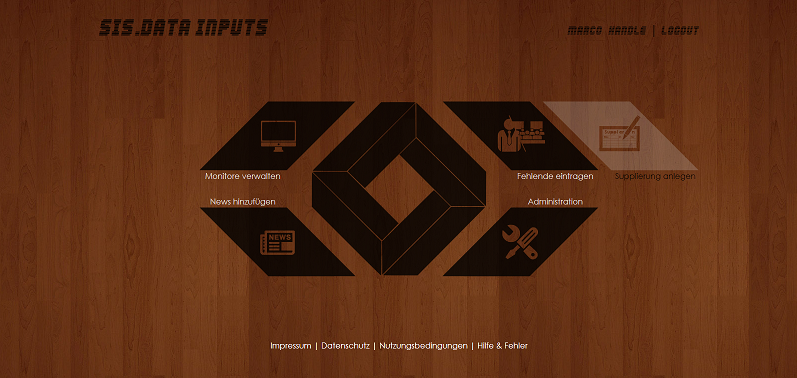
\includegraphics[keepaspectratio=true, width=17cm]{images/screenshots/data-inputs_substitudes.png}
\caption{Data-Input-Menü}
\label{fig:instr_substitudes_dataInput}
\end{figure}
\begin{figure}[H]
\centering
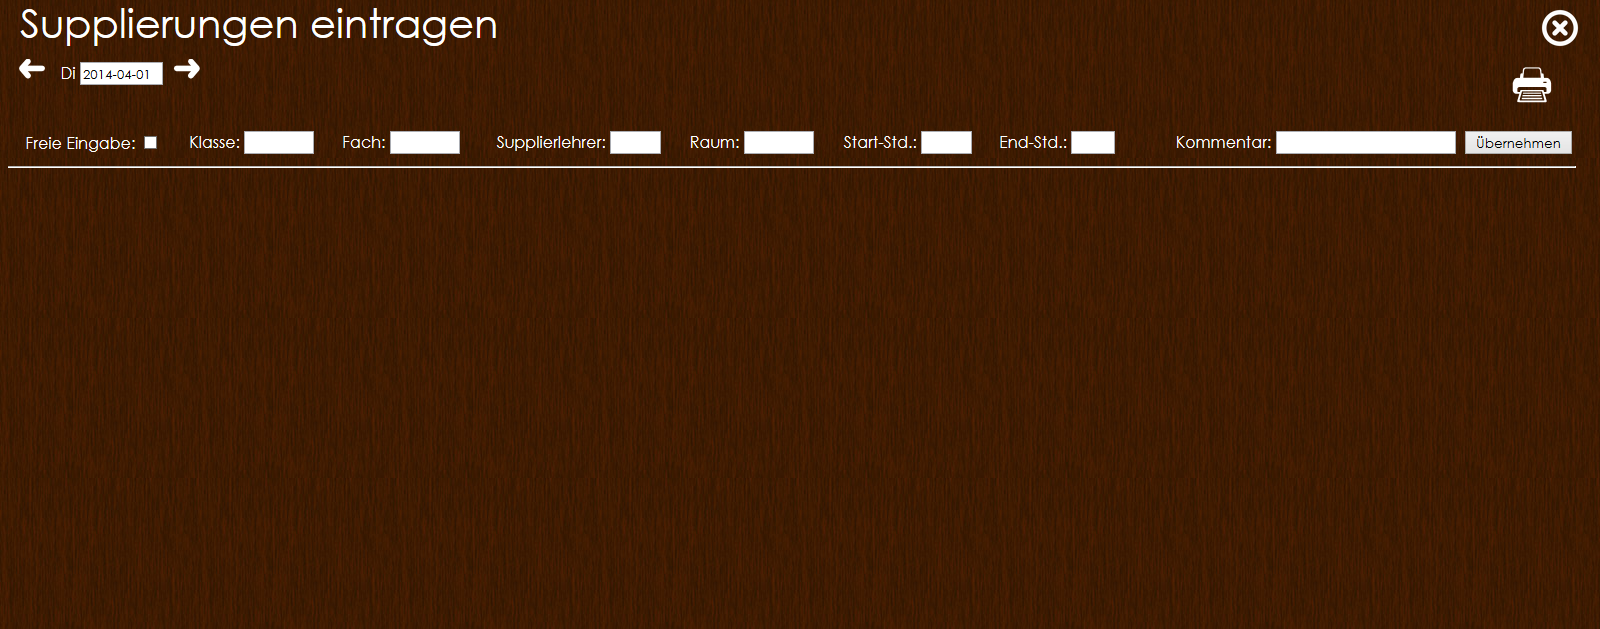
\includegraphics[keepaspectratio=true, width=17cm]{images/screenshots/substitudes_nofree.png}
\caption{Eingabemaske normal}
\label{fig:instr_substitudes_subNoFree}
\end{figure}
\begin{figure}[H]
\centering
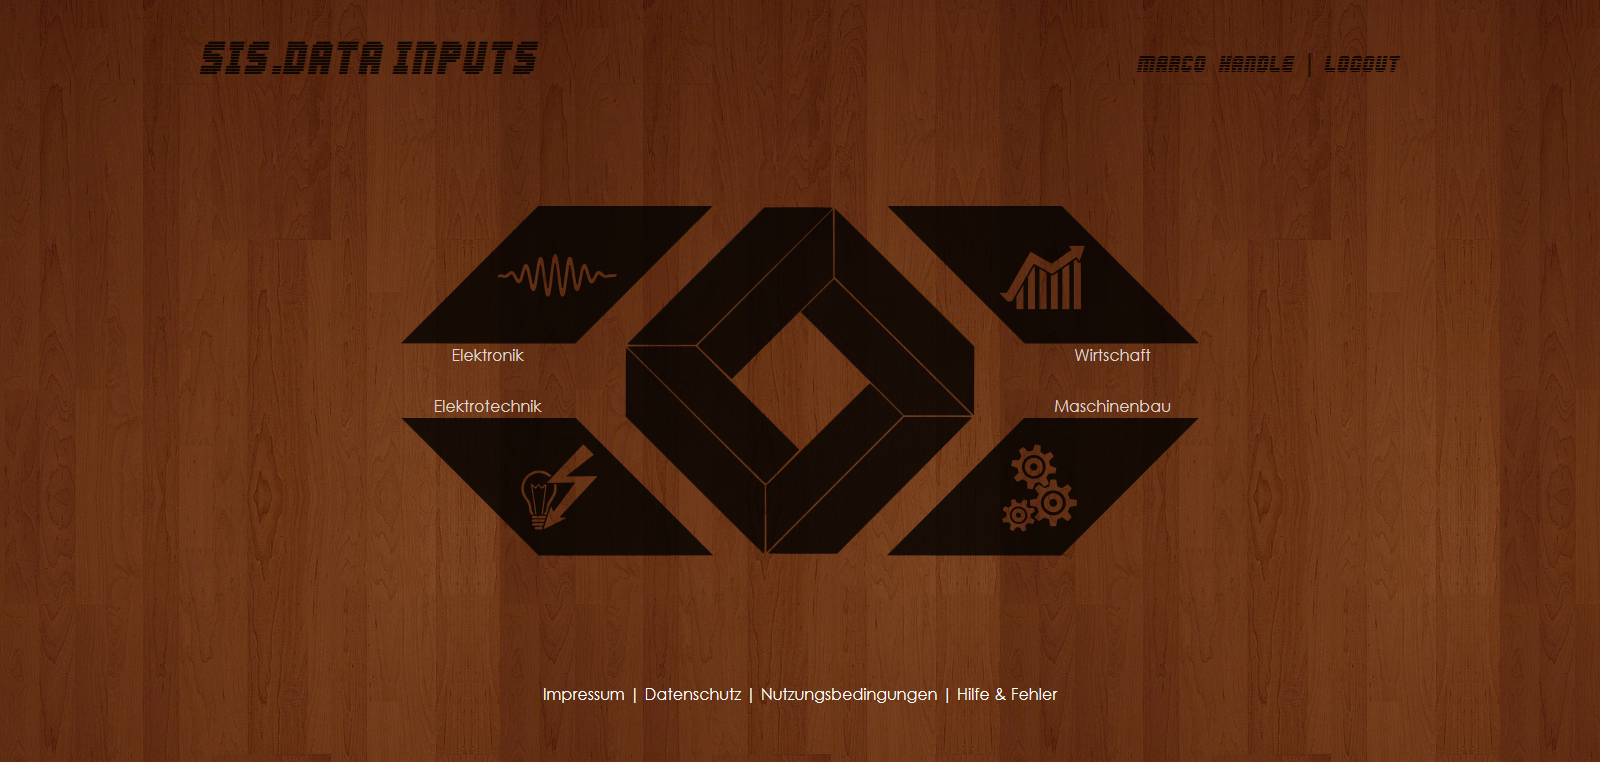
\includegraphics[keepaspectratio=true, width=17cm]{images/screenshots/substitudes_sections.png}
\caption{Super User Auswahl}
\label{fig:instr_substitudes_subSuUs}
\end{figure}
Es gibt 4 grundlegende Eingabevarianten:
\begin{itemize}
	\item Normale Eingabe\\
		siehe \autoref{sec:instr_admin_sub_noFree}
	\item Freie Eingabe\\
		siehe \autoref{sec:instr_admin_sub_Free}
		\begin{itemize}
			\item Stunde verschieben\\
				siehe \autoref{sec:instr_admin_sub_move}
			\item Stunde hinzufügen\\
				siehe \autoref{sec:instr_admin_sub_add}
			\item Stunde entfällt\\
				siehe \autoref{sec:instr_admin_sub_remove}
		\end{itemize}
\end{itemize}
\subsection{Normale Eingabe}\label{sec:instr_admin_sub_noFree}
Diese Eingabemethode (siehe \autoref{fig:instr_substitudes_subNoFree}) dient zur Erfassung von Supplierstunden von Klassen, deren Lehrer vorher als fehlend definiert wurde. Fehlen mehrere Lehrer in einer Klasse zur selben Zeit (Labor, FTKL, ...) ist die Freie Eingabe (siehe \autoref{sec:instr_admin_sub_Free}) zu verwenden.
\begin{table}[H]
\centering
\begin{tabular}{p{3 cm}p{6 cm}p{5 cm}}
   \toprule
   \textbf{Eingabefeld} & \textbf{Typ} & \textbf{Wertebereich} \\
   \midrule
          Freie Eingabe & Checkbox \newline nicht genutzt & \\
          \hline
          \textbf{Klasse} & Listenfeld - Pflichtfeld & Abteilungs-abhängig \\
          \hline
          Fach & Listenfeld - optional & \\
          \hline
          \textbf{Supplierlehrer} & Listenfeld - Pflichtfeld & \\
          \hline
          Raum & Listenfeld - optional & \\
          \hline
          \textbf{Start-Std.} & Erste Schulstunde der Supplierung  -Pflichtfeld & 1-16 \\
		  \hline
          \textbf{End-Std.} & Letzte Schulstunde der Supplierung  -Pflichtfeld & 1-16 \newline größer oder gleich Start-Std.\\
          \hline
          Kommentar & Textfeld - optional & \\
   \bottomrule
\end{tabular}
\caption{Eingabefelder normale Eingabe}
\end{table}
Mit der Schaltfläche Übernehmen wird eine Plausibilitätsüberprüfung vorgenommen und bei fehlerfreier Eingabe die Supplierstunde übernommen. Bei einer Fehleingabe wird der Fehler angezeigt und muss korrigiert werden. Nach der korrekten Übernahme wird die Checkbox Löschen in der erfassten Eingabezeile eingeblendet.
\subsection{Freie Eingabe} \label{sec:instr_admin_sub_Free}
Mit der Freien Eingabe können auch Supplierstunden erfasst werden, wenn der ursprüngliche Lehrer nicht fehlt. Um diese Methode auszuwählen muss in der Eingabemaske die Checkbox Freie Eingabe gesetzt werden. Es erscheinen zusätzliche Eingabefelder und drei Radio-Buttons zur Auswahl der Eingabemethode.\\
Standardmäßig ist der Radio-Button Verschiebung ausgewählt. Bei einer anderen Wahl ändern sich die Eingabefelder.
\subsubsection{Verschieben von Schulstunden} \label{sec:instr_admin_sub_move}
Diese Eingabemethode dient dazu:
\begin{itemize}
	\item Schulstunden einer Klasse innerhalb eines Tages zu verschieben
	\item Supplierstunden von 2 oder mehreren fehlenden Lehrern zu erfassen (Vertretung)
	\item Mehrstündige Fächer zu kürzen
\end{itemize}
Zur normalen Eingabemaske sind 3 zusätzliche Felder zu erfassen (siehe \autoref{fig:instr_substitudes_subMove}).
\begin{table}[H]
\centering
\begin{tabular}{p{3 cm}p{6 cm}p{5 cm}}
   \toprule
   \textbf{Eingabefeld} & \textbf{Typ} & \textbf{Wertebereich} \\
   \midrule
          \textbf{Freie Eingabe} & Checkbox \newline gesetzt & \\
          \hline
          \textbf{Klasse} & Listenfeld - Pflichtfeld & Abteilungs-abhängig \\
          \hline
          Fach & Listenfeld - optional & \\
          \hline
          Supplierlehrer & Listenfeld - Optional & \\
          \hline
          Raum & Listenfeld - optional & \\
          \hline
          \textbf{Start-Std.} & Erste Schulstunde der Supplierung  -Pflichtfeld & 1-16 \\
		  \hline
          \textbf{End-Std.} & Letzte Schulstunde der Supplierung  -Pflichtfeld & 1-16 \newline größer oder gleich Start-Std.\\
          \hline
          Kommentar & Wird automatisch mit \enquote{Verschiebung von} befüllt & \\
          \hline
          \textbf{Radio-Button} & \textbf{Verschiebung} - gesetzt\newline Hinzufügen - nicht gesetzt \newline Entfällt - nicht gesetzt & \\
          \hline
          \textbf{Urs. Start-Std.} & Erste ursprüngliche Schulstunde der Supplierung  -Pflichtfeld & 1-16 \\
          \hline
          \textbf{Urs. End-Std.} & Letzte ursprüngliche Schulstunde der Supplierung  -Pflichtfeld & 1-16 \newline größer oder gleich Urs. Start-Std.\\
          \hline
          Urs. Lehrer & Listenfeld - Optional \newline ursprünglicher Lehrer der Supplierung\\
   \bottomrule
\end{tabular}
\caption{Eingabefelder Verschiebung}
\end{table}
Einige der optionalen Informationen werden automatisch mit den Daten der ursprünglichen Stunde befüllt. Der ursprüngliche Lehrer kann/muss aber nicht angegeben werden. Wird er nicht angegeben, werden alle Stunden, die die Klasse zu der angegebenen Zeit hat, verschoben. Wenn die Klasse geteilt ist, alle Teilungen auch.\\
Mit der Schaltfläche Übernehmen wird eine Plausibilitätsüberprüfung durchgeführt und bei fehlerfreier Eingabe übernommen. Bei einer Fehleingabe wird der Fehler angezeigt und muss korrigiert werden. Nach der korrekten Übernahme wird die Checkbox Löschen in der erfassten Eingabezeile eingeblendet.
\begin{figure}[H]
\centering
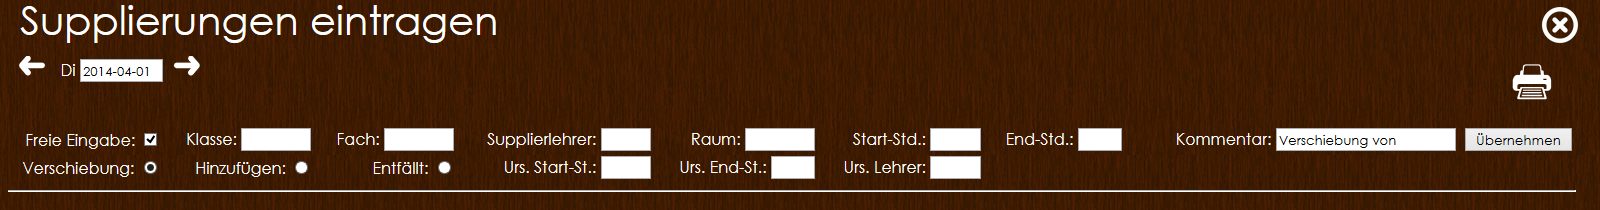
\includegraphics[keepaspectratio=true, width=17cm]{images/screenshots/substitudes_move.png}
\caption{Eingabemaske Verschiebung}
\label{fig:instr_substitudes_subMove}
\end{figure}
\subsubsection{Hinzufügen}\label{sec:instr_admin_sub_add}
Diese Eingabemethode dient dazu, zusätzliche Schulstunden an einem Tag einzufügen. Der neue Eintrag überschreibt den ursprünglichen Stundenplan der Klasse für diesen Tag.\\
Die Eingabemaske entspricht jener der Normalen Eingabe und enthält zusätzlich die Radio-Buttons (siehe \autoref{fig:instr_substitudes_subAdd}).
\begin{table}[H]
\centering
\begin{tabular}{p{3 cm}p{6 cm}p{5 cm}}
   \toprule
   \textbf{Eingabefeld} & \textbf{Typ} & \textbf{Wertebereich} \\
   \midrule
          \textbf{Freie Eingabe} & Checkbox \newline gesetzt & \\
          \hline
          \textbf{Klasse} & Listenfeld - Pflichtfeld & Abteilungs-abhängig \\
          \hline
          \textbf{Fach} & Listenfeld - optional & \\
          \hline
          \textbf{Supplierlehrer} & Listenfeld - Pflichtfeld & \\
          \hline
          Raum & Listenfeld - optional & \\
          \hline
          \textbf{Start-Std.} & Erste Schulstunde  -Pflichtfeld & 1-16 \\
		  \hline
          \textbf{End-Std.} & Letzte Schulstunde -Pflichtfeld & 1-16 \newline größer oder gleich Start-Std.\\
          \hline
          Kommentar & Textfeld - optional & \\
          \hline
          \textbf{Radio-Button} & Verschiebung - nicht gesetzt\newline 
          \textbf{Hinzufügen} - gesetzt \newline Entfällt - nicht gesetzt & \\
   \bottomrule
\end{tabular}
\caption{Eingabefelder Hinzufügen}
\end{table}
Mit der Schaltfläche Übernehmen wird eine Plausibilitätsüberprüfung durchgeführt und bei fehlerfreier Eingabe übernommen. Bei einer Fehleingabe wird der Fehler angezeigt und muss korrigiert werden. Nach der korrekten Übernahme wird die Checkbox Löschen in der erfassten Eingabezeile eingeblendet.
\begin{figure}[H]
\centering
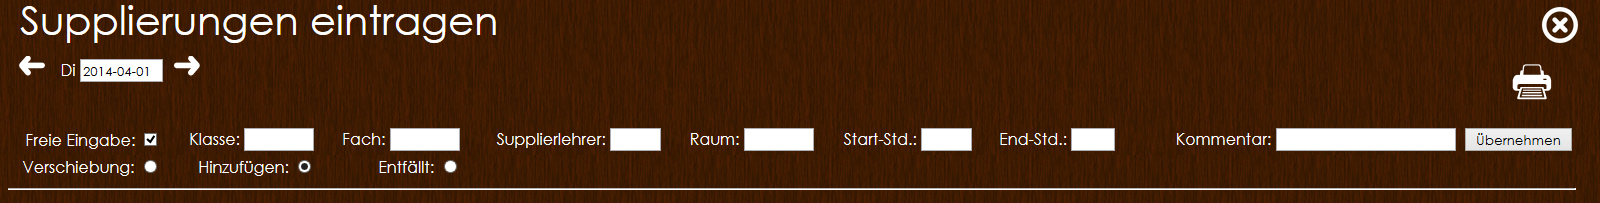
\includegraphics[keepaspectratio=true, width=17cm]{images/screenshots/substitudes_add.png}
\caption{Eingabemaske Hinzufügen}
\label{fig:instr_substitudes_subAdd}
\end{figure}
\subsubsection{Entfallen}\label{sec:instr_admin_sub_remove}
Entfällt eine Schulstunden ersatzlos, ist der Radio-Button Entfällt zu setzen. Die angegebene Stunde wird im Stundenplan der Schüler und Lehrer gelöscht.\\
Die Eingabemaske wird auf die unbedingt notwendigen Felder reduziert (siehe \autoref{fig:instr_substitudes_subRemove}).
\begin{table}[H]
\centering
\begin{tabular}{p{3 cm}p{6 cm}p{5 cm}}
   \toprule
   \textbf{Eingabefeld} & \textbf{Typ} & \textbf{Wertebereich} \\
   \midrule
          \textbf{Freie Eingabe} & Checkbox \newline gesetzt & \\
          \hline
          \textbf{Klasse} & Listenfeld - Pflichtfeld & Abteilungs-abhängig \\
          \hline
          Kommentar & Wird automatisch mit \enquote{entfällt} befüllt & \\
          \hline
          \textbf{Radio-Button} & Verschiebung - nicht gesetzt\newline Hinzufügen - nicht gesetzt \newline \textbf{Entfällt} - gesetzt & \\
          \hline
          \textbf{Urs. Start-Std.} & Erste ursprüngliche Schulstunde die Entfällt  -Pflichtfeld & 1-16 \\
          \hline
          \textbf{Urs. End-Std.} & Letzte ursprüngliche Schulstunde die Entfällt  -Pflichtfeld & 1-16 \newline größer oder gleich Urs. Start-Std.\\
          \hline
          \textbf{Urs. Lehrer} & Listenfeld - Pflichtfeld \newline ursprünglicher Lehrer der entfallenen Schulstunde\\
   \bottomrule
\end{tabular}
\caption{Eingabefelder Entfällt}
\end{table}
Mit der Schaltfläche Übernehmen wird eine Plausibilitätsüberprüfung durchgeführt und bei fehlerfreier Eingabe übernommen. Bei einer Fehleingabe wird der Fehler angezeigt und muss korrigiert werden. Nach der korrekten Übernahme wird die Checkbox Löschen in der erfassten Eingabezeile eingeblendet.
\begin{figure}[H]
\centering
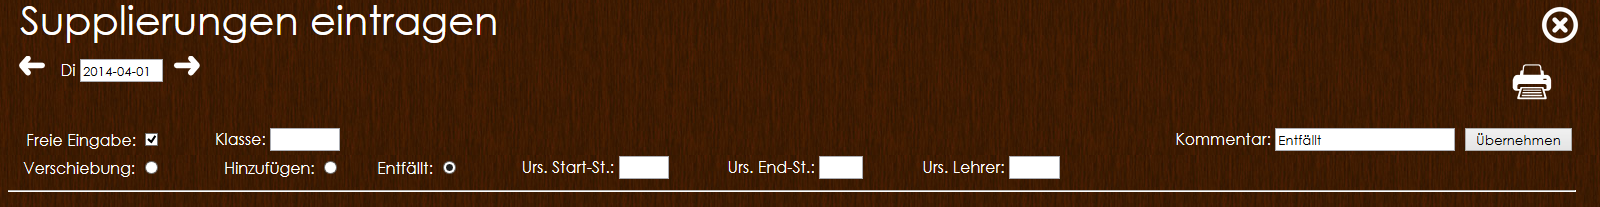
\includegraphics[keepaspectratio=true, width=17cm]{images/screenshots/substitudes_remove.png}
\caption{Eingabemaske Entfallen}
\label{fig:instr_substitudes_subRemove}
\end{figure}
\subsection{Fehler}
Wird in einem Eingabefeld ein Wert eingegeben, der nicht in der angezeigten Liste vorkommt oder nicht im Wertebereich liegt, wird ein Fehler zurückgegeben. In einem Pop-Up wird der Name des fehlerhaften Eingabefeldes angezeigt. Das Pop-Up ist mit der Schaltfläche Ok zu bestätigen. Anschließend muss die Eingabe erneut erfolgen.\\
Eine weitere Fehlerquelle kann darin liegen, dass bei der Normalen Eingabe (siehe \autoref{sec:instr_admin_sub_noFree}) zur Erfassung einer Supplierung ein ursprünglicher Lehrer gewählt wird, der nicht als fehlend erfasst wurde oder wenn die ursprüngliche Stunde nicht gefunden wird. Diese Fehler werden unter der Seitenüberschrift angezeigt und die Trennlinie unter der Eingabezeile wird rot (siehe \autoref{fig:instr_substitudes_fail}).
\begin{figure}[H]
\centering
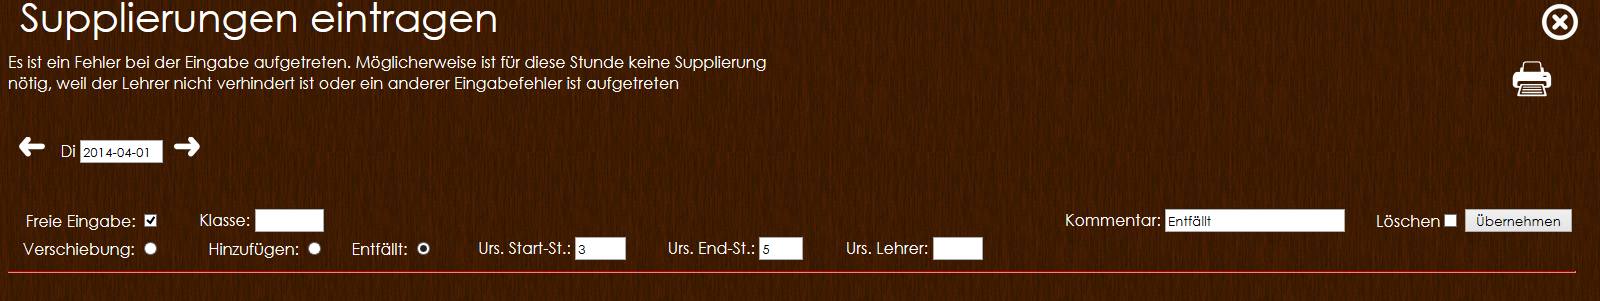
\includegraphics[keepaspectratio=true, width=17cm]{images/screenshots/substitudes_fail.png}
\caption{Fehleingabe}
\label{fig:instr_substitudes_fail}
\end{figure}
\subsection{Einträge ändern}
Bestehende Einträge können durch überschreiben geändert werden. Die Änderungen werden nach dem Drücken auf die Schaltfläche Übernehmen der Eingabezeile übernommen, sofern kein Fehler auftritt. Bei einer Fehlermeldung ist die Eingabe entsprechend zu korrigieren.
\subsection{Löschen}
Das Löschen eines Eintrages erfolgt über die Checkbox Löschen der entsprechenden Eingabezeile. Diese muss gesetzt und dann mit Übernehmen bestätigt werden. Es erfolgt keine weitere Sicherheitsabfrage und ist der Eintrag unwiderruflich gelöscht

\newpage
\section{Administrative Eingaben}

Alle im folgendem beschriebenen Eingaben (siehe \autoref{fig:instr_other_menu}) sind ausschließlich für den Super-User sichtbar. Der Einstieg erfolgt über den Punkt Administrator im Menü „Data-Input“.
\begin{figure}[H]
\centering
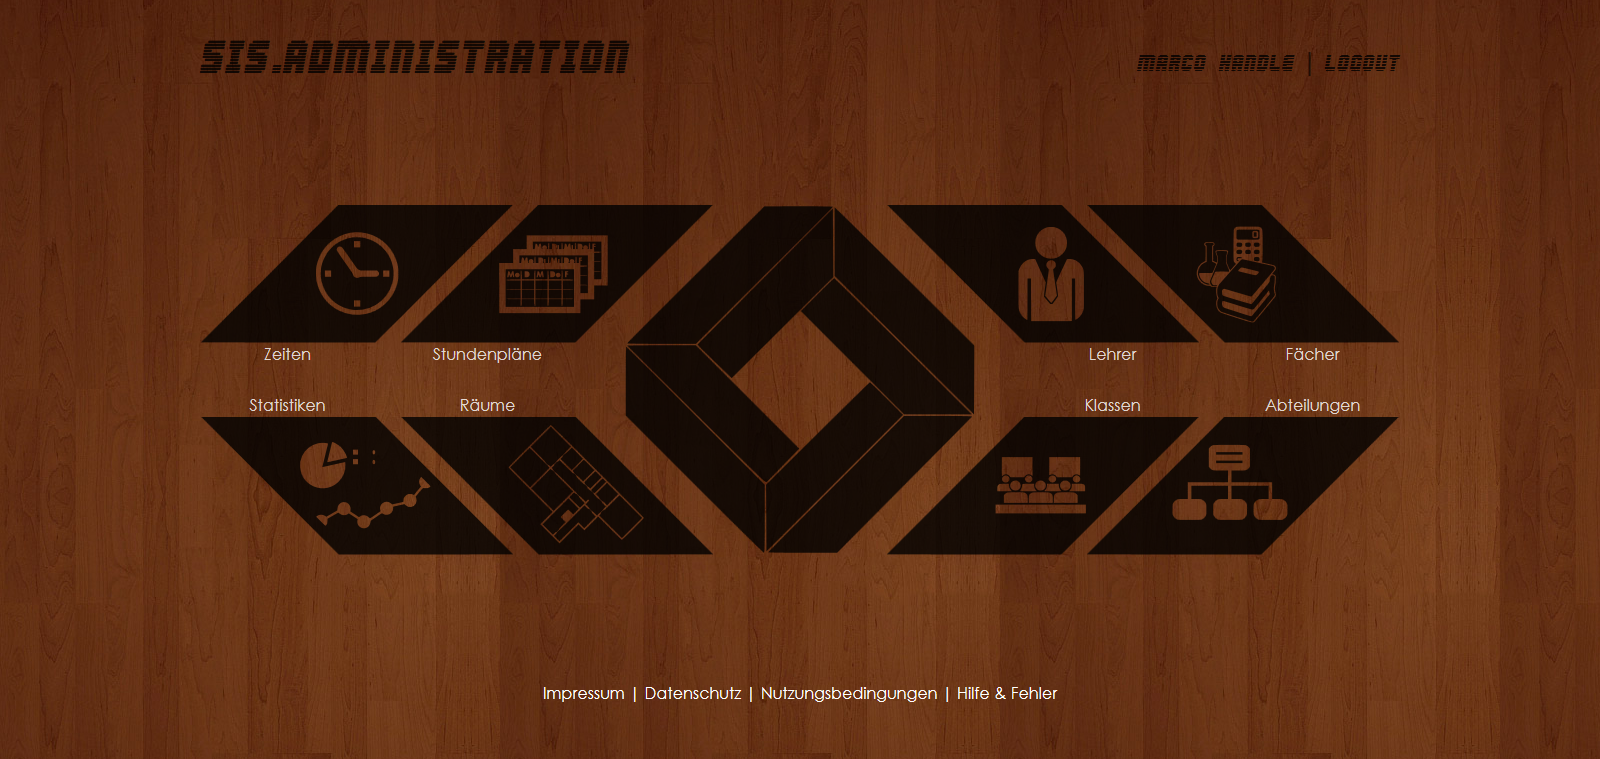
\includegraphics[keepaspectratio=true, width=17cm]{images/screenshots/admin_menu.png}
\caption{Administrationsmenü}
\label{fig:instr_other_menu}
\end{figure}
\subsection{Stunden}\label{sec:instr_other_hours}
Standardmäßig sind 16 Schulstunden mit der jeweiligen Start- und Endzeit für jeden Wochentag (Montag bis Freitag) angelegt (siehe \autoref{fig:instr_other_hours}). Über die Schaltfläche am linken bzw. rechten Seitenrand kann zwischen den Wochentagen gewechselt werden. Die Anzeige der Stunden wird entsprechend angepasst.\\
Die Änderungen können nun in den Eingabezeilen vorgenommen oder auch eine weitere Stunde angefügt werden. Alle Eingabefelder sind Pflichtfelder. Die Übernahme erfolgt mit der Schaltfläche Übernehmen in der jeweiligen Eingabezeile.\\
Aus Gründen der Datenkonsistenz der Stunden- und Supplierpläne ist das Löschen von Stunden nicht möglich.
\begin{figure}[H]
\centering
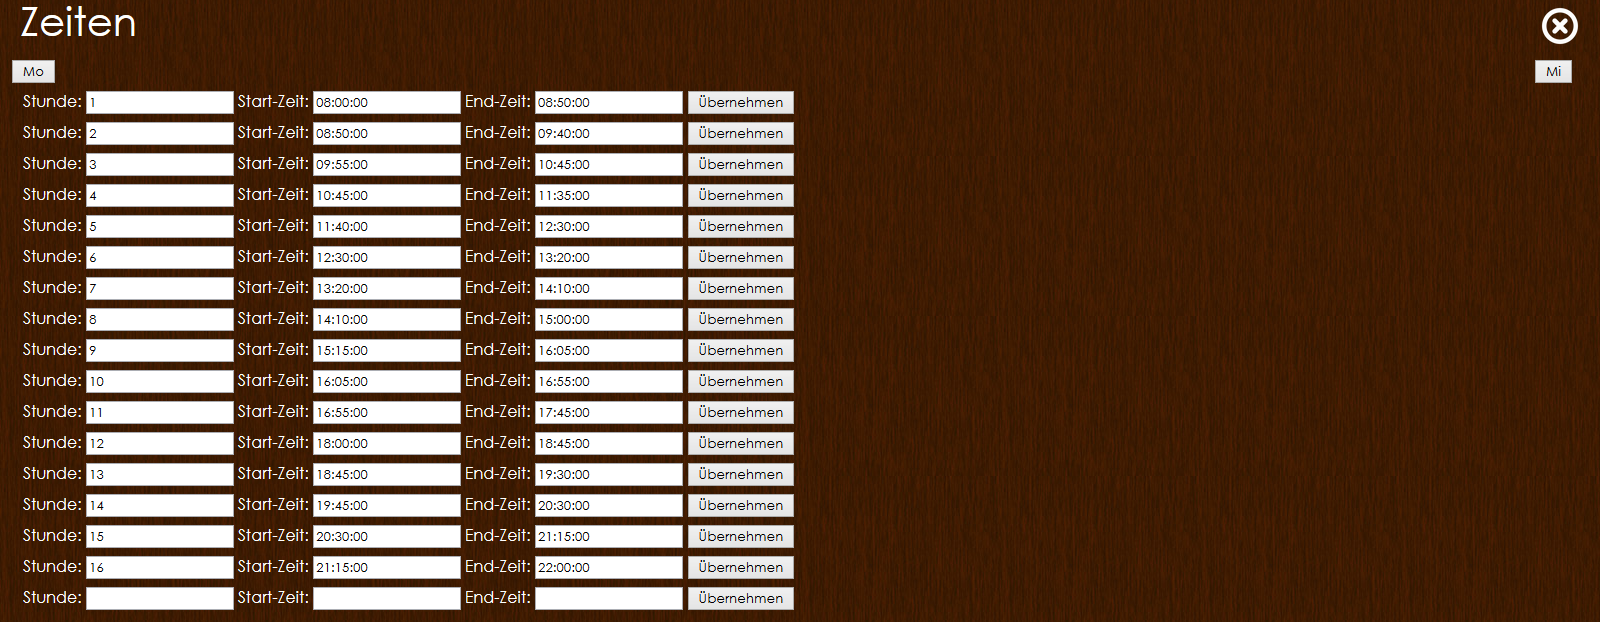
\includegraphics[keepaspectratio=true, width=17cm]{images/screenshots/hours_input.png}
\caption{Stunden bearbeiten}
\label{fig:instr_other_hours}
\end{figure}
\subsection{Stundenpläne}
Für die Erfassung eines Stundenplanes muss zuerst die Klasse (Listenfeld) und der Wochentag (Listenfeld) ausgewählt werden. Die Auswahl des Wochentages ist mit der Schaltfläche OK zu bestätigen (siehe \autoref{fig:instr_other_timetables_menu}). Ist bereits ein Stundenplan für den Tag vorhanden, wird dieser geladen (siehe \autoref{fig:instr_other_timetables_layout}). Über die Schaltfläche am linken bzw. rechten Seitenrand kann zwischen den Wochentagen gewechselt werden. Die Anzeige der Stunden wird entsprechend angepasst (siehe \autoref{fig:instr_other_timetables_day}).
Links oben werden die Klasse und der Wochentag angezeigt. Mit einem Klick auf die Klasse kehrt man ins Menü für die Auswahl der Klasse zurück (siehe \autoref{fig:instr_other_timetables_infos}).
\begin{figure}[H]
\centering
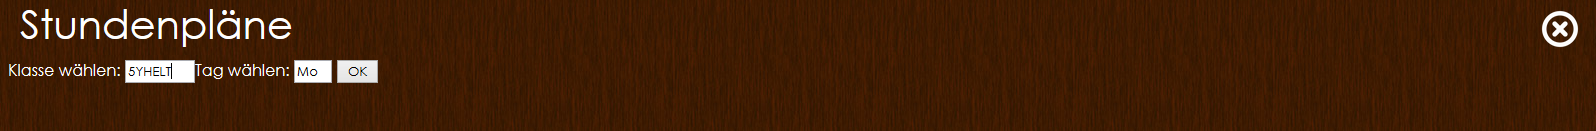
\includegraphics[keepaspectratio=true, width=17cm]{images/screenshots/timetables_input_menu.png}
\caption{Stundenplan auswählen}
\label{fig:instr_other_timetables_menu}
\end{figure}
\begin{figure}[H]
\centering
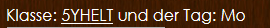
\includegraphics[keepaspectratio=true, width=6cm]{images/screenshots/timetables_input_infos.png}
\caption{Klasse und Tag}
\label{fig:instr_other_timetables_infos}
\end{figure}
\begin{figure}[H]
\centering

\includegraphics[keepaspectratio=true, width=17cm]{images/screenshots/timetables_input_day.png}
\caption{Tagauswahl}
\label{fig:instr_other_timetables_day}
\end{figure}
\begin{figure}[H]
\centering
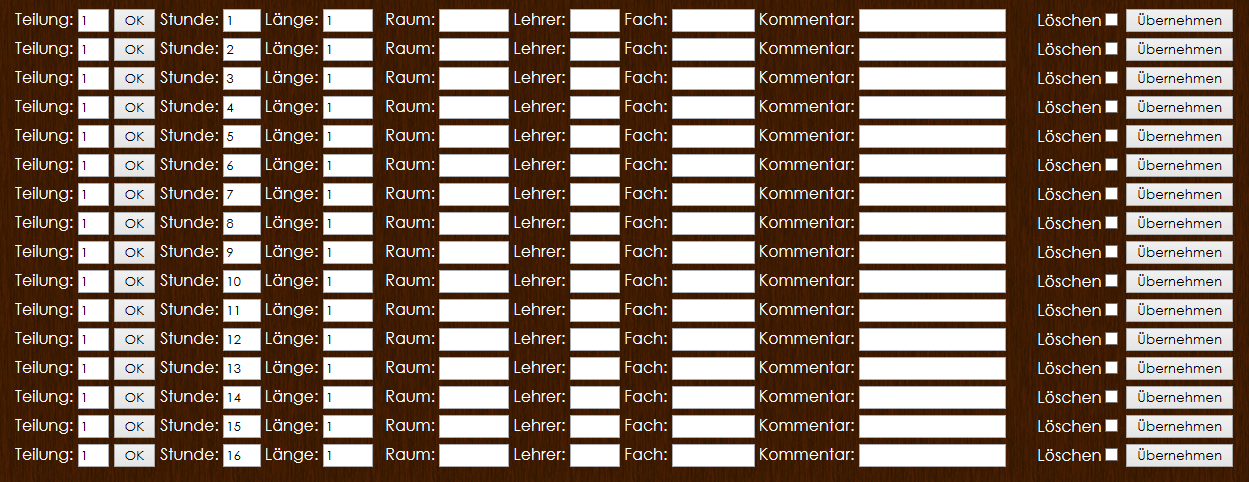
\includegraphics[keepaspectratio=true, width=17cm]{images/screenshots/timetables_input_layout.png}
\caption{Eingabemaske}
\label{fig:instr_other_timetables_layout}
\end{figure}
\subsubsection{Einstündiges Fach} \label{sec:instr_other_timetables_single}
Über die Standardeinstellung können Einzelstunden erfasst werden. In der entsprechenden Schulstunde sind der Lehrer und das Fach anzugeben.
\begin{table}[H]
\centering
\begin{tabular}{p{3 cm}p{10 cm}}
   \toprule
   \textbf{Eingabefeld} & \textbf{Typ} \\
   \midrule
          Teilung & \textbf{1} \newline nicht ändern \\
          \hline
          OK & Schaltfläche \\
          \hline
          Stunde & Schulstunde \newline Kann nicht geändert werden\\
          \hline
          Länge & \textbf{1} \newline Nicht ändern \\
          \hline
          Raum & Listenfeld - optional \\
          \hline
          \textbf{Lehrer} & Listenfeld - Pflichtfeld \\
		  \hline
          \textbf{Fach} & Listenfeld - Pflichtfeld.\\
          \hline
          Kommentar & Textfeld - optional \\
          \hline
          Löschen & Checkbox - \textbf{nicht gesetzt}\\
   \bottomrule
\end{tabular}
\caption{Eingabefelder Stundenplan}
\end{table}
Die Änderungen bzw. Ergänzungen sind mit der Schaltfläche Übernehmen in der jeweiligen Eingabezeile zu übernehmen (siehe \autoref{fig:instr_other_timetables_singleHour}).
\begin{figure}[H]
\centering

\includegraphics[keepaspectratio=true, width=17cm]{images/screenshots/timetables_input_singleHour.png}
\caption{Beispiel Einzelstunde}
\label{fig:instr_other_timetables_singleHour}
\end{figure}
\subsubsection{Mehrstündiges Fach}
Die Eingabe erfolgt analog zu jener im \autoref{sec:instr_other_timetables_single} beschriebenen. Es ist aber im Eingabefeld Länge die Anzahl der zusammenhängenden Schulstunden anzugeben. Wird nun in ein anderes Eingabefeld gewechselt, werden die nachfolgenden Eingabezeilen ausgeblendet, welche durch das mehrstündige Fach abgedeckt werden (siehe \autoref{fig:instr_other_timetables_multiHour}).\\
Wird zum Beispiel in der ersten Stunde ein Fach mit der Länge von 3 Stunden eingetragen, werden die Eingabezeilen der zweiten und dritte Stunde ausgeblendet.\\
Eingaben und Änderungen müssen jeweils durch das Drücken auf die Schaltfläche Übernehmen übernommen werden.
\begin{figure}[H]
\centering
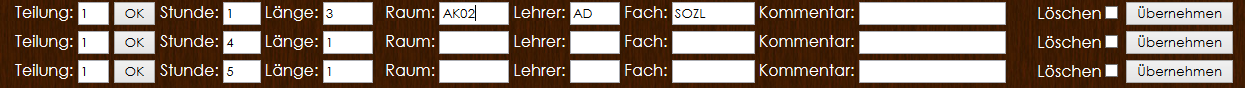
\includegraphics[keepaspectratio=true, width=17cm]{images/screenshots/timetables_input_multiHour.png}
\caption{Beispiel Mehrstündiger Unterricht}
\label{fig:instr_other_timetables_multiHour}
\end{figure}
\subsubsection{Teilung von Klassen}
Wird eine Klasse im Unterricht geteilt, ist dies über das Eingabefeld Teilung zu erfassen. Es ist zu beachten, dass die geteilten Fächer gleich lang sein müssen. Sind die geteilten Fächer ungleich lang, so ist der Rest der längeren Teilung als Einzelstunde zu erfassen. Eine Klasse kann maximal in 7 Teile geteilt werden.\\
Um eine Teilung erfassen zu können, ist im Eingabefeld Teilung die Anzahl der Teilungen einzugeben und mit der Schaltfläche OK zu bestätigen. Anschließend erscheinen weitere Eingabezeilen (siehe \autoref{fig:instr_other_timetables_divide7}).\\
Die Eingabe erfolgt sinngemäß wie die Erfassung eines mehrstündigen Fachs. Jede einzelne Eingabezeile der Teilung ist mit der Schaltfläche Übernehmen zu bestätigen.
\begin{figure}[H]
\centering
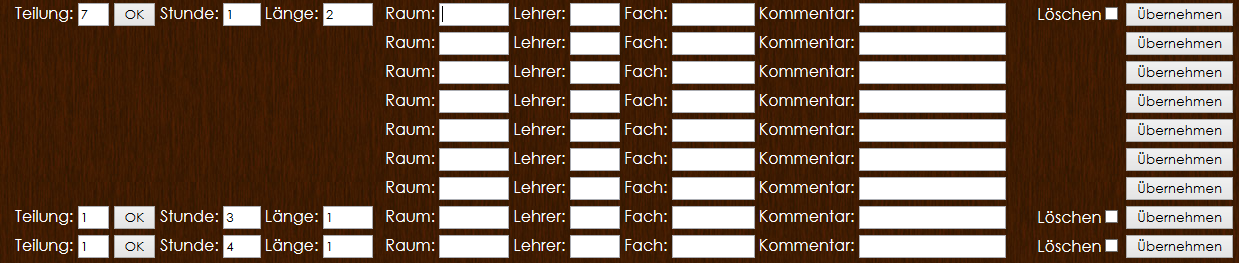
\includegraphics[keepaspectratio=true, width=17cm]{images/screenshots/timetables_input_divide7.png}
\caption{Beispiel Teilungen}
\label{fig:instr_other_timetables_divide7}
\end{figure}
Jede eigene Zeile muss mit Übernehmen bestätigt werden. Gelöscht kann jedoch nur ein ganzer Block werden. Dies muss mit einem Hacken bei Löschen und anschließendem Klicken auf Übernehmen erfolgen.
\subsubsection{Löschen von Unterrichtsstunden}
Das Löschen von Einträgen kann einzeln über die Checkbox Löschen vorgenommen werden. Der Stundenplan eines Tages kann über die Schaltfläche \enquote{Stundenplan löschen} \textbf{unwiderruflich} gelöscht werden (siehe \autoref{fig:instr_other_timetables_delete}).
\begin{figure}[H]
\centering

\includegraphics[keepaspectratio=true, width=5cm]{images/screenshots/timetables_input_delete.png}
\caption{Löschen}
\label{fig:instr_other_timetables_delete}
\end{figure}
\subsection{Lehrer}
Dieser Punkt ist dazu da, dass man Lehrer bearbeiten und hinzufügen kann. Auch hier ist es nicht möglich Lehrer zu löschen, da es wie bei Stunden zu großen Problemen kommen kann. (siehe \autoref{sec:instr_other_hidden})\\
Im Feld Name muss der vollständige Name des Lehrers eingegeben werden, im Feld Kürzel wird das Lehrer-Kürzel eingetragen, im Feld Kurzname muss ein verkürzter Name eingegeben werden, dieser wird zum Beispiel bei den Supplierungen am Display angezeigt. Im Feld Stammabteilung kann eine Abteilung eingegeben werden, dies ist jedoch optional, da nicht jeder Lehrer eine Stammabteilung hat. Wie schon erwähnt ist der Hacken für unsichtbar zum stilllegen eines Lehrers gut. (Eingabemaske siehe \autoref{fig:instr_other_teacher}) Sollen vorhandene Daten geändert werden, so kann man den vorhandenen Lehrer abändern und mit Übernehmen speichern.
\begin{figure}[H]
\centering

\includegraphics[keepaspectratio=true, width=17cm]{images/screenshots/teachers_input.png}
\caption{Eingabemaske Lehrer}
\label{fig:instr_other_teacher}
\end{figure}
\subsection{Fächer}
Über diese Eingabemaske werden Lehrereinträge bearbeitet und hinzugefügt (siehe \autoref{fig:instr_other_subjects}). Aus Gründen der Datenkonsistenz der Stunden- und Supplierpläne ist das Löschen von Lehrern nicht möglich.
\begin{table}[H]
\centering
\begin{tabular}{p{3 cm}p{10 cm}}
   \toprule
   \textbf{Eingabefeld} & \textbf{Typ} \\
   \midrule
          \textbf{Name} & Textfeld - Pflichtfeld \newline vollständiger Name \\
          \hline
          \textbf{Kürzel} & Textfeld - Pflichtfeld \newline Lehrer-Kürzel \\
          \hline
          \textbf{Kurzname} & Textfeld - Pflichtfeld \newline Kurzname für die Anzeige am Display \\
          \hline
          Stammabteilung & Textfeld - optional \\
          \hline
          Unsichtbar & Checkbox \\
   \bottomrule
\end{tabular}
\caption{Eingabefelder Fächer}
\end{table}
Wird die Checkbox Unsichtbar bei einem Lehrer gesetzt, wird dieser in den Listenfelder nicht mehr angezeigt. (siehe \autoref{sec:instr_other_hidden})\\
Änderungen und Ergänzungen sind über die Schaltfläche Übernehmen in den Eingabezeilen zu bestätigen.
\begin{figure}[H]
\centering
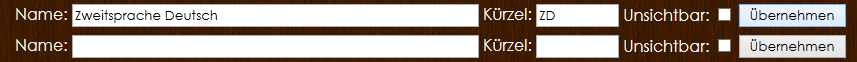
\includegraphics[keepaspectratio=true, width=17cm]{images/screenshots/subjects_input.png}
\caption{Eingabemaske Fächer}
\label{fig:instr_other_subjects}
\end{figure}
\subsection{Statistiken}
Um die Akzeptanz der Anwendung beurteilen zu können, wurde ein Statistikmodul implementiert, obwohl dies im vorgegebenen Pflichtenheft nicht vorgesehen ist. Es werden deshalb unter anderem anonymisiert die Zugriffe auf die verschiedenen Seiten, von welchen Endgeräten die Zugriffe erfolgen, welche Schulstufen, etc. registriert und in Grafiken ausgewertet.
\begin{figure}[H]
\centering
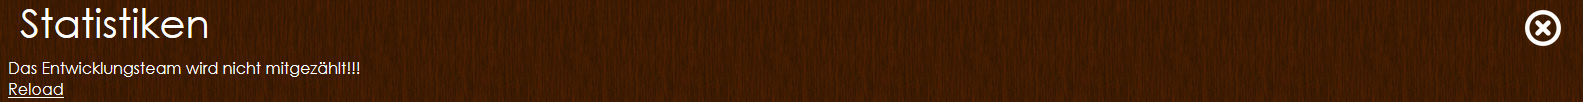
\includegraphics[keepaspectratio=true, width=17cm]{images/screenshots/statistics_header.png}
\caption{Statistiken Reload}
\label{fig:instr_other_statistics_header}
\end{figure}
\subsubsection{Browser PC}
In dieser Statistik sind die Browser der Geräte dargestellt, welche die PC Seiten aufrufen. (siehe \autoref{fig:instr_other_statistics_browser_PC})
\begin{figure}[H]
\centering
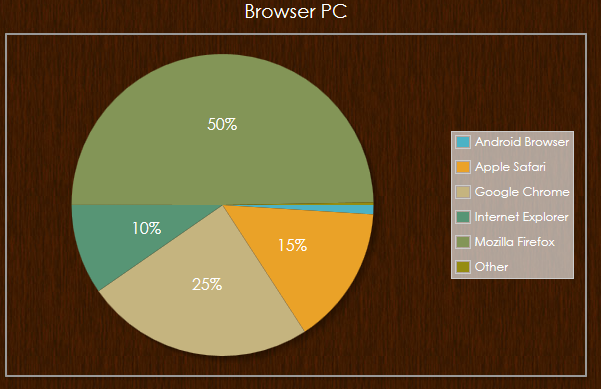
\includegraphics[keepaspectratio=true, width=8cm]{images/screenshots/statistics_browser_PC.png}
\caption{Browser PC}
\label{fig:instr_other_statistics_browser_PC}
\end{figure}
\subsubsection{Geräte PC}
In dieser Statistik sind die Geräte bzw. Betriebssysteme der Geräte dargestellt, welche die PC Seiten aufrufen. (siehe \autoref{fig:instr_other_statistics_os_PC})
\begin{figure}[H]
\centering
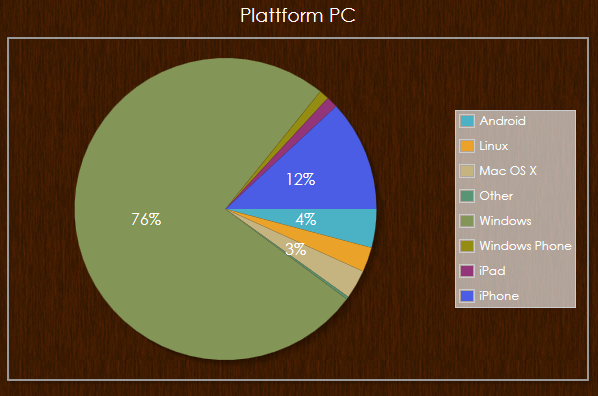
\includegraphics[keepaspectratio=true, width=8cm]{images/screenshots/statistics_os_PC.png}
\caption{Geräte PC}
\label{fig:instr_other_statistics_os_PC}
\end{figure}
\subsubsection{Browser Mobil}
In dieser Statistik sind die Browser der Geräte dargestellt, welche die App aufrufen. (siehe \autoref{fig:instr_other_statistics_browser_Mob})
\begin{figure}[H]
\centering
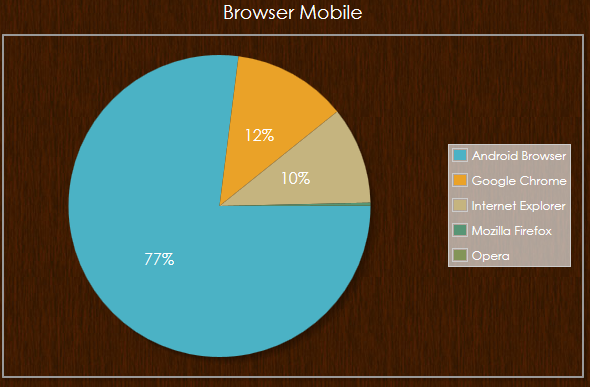
\includegraphics[keepaspectratio=true, width=8cm]{images/screenshots/statistics_browser_Mob.png}
\caption{Browser Mobil}
\label{fig:instr_other_statistics_browser_Mob}
\end{figure}
\subsubsection{Geräte Mobil}
In dieser Statistik sind die Geräte bzw. Betriebssysteme der Geräte dargestellt, welche die App Seiten aufrufen. (siehe \autoref{fig:instr_other_statistics_os_Mob})
\begin{figure}[H]
\centering
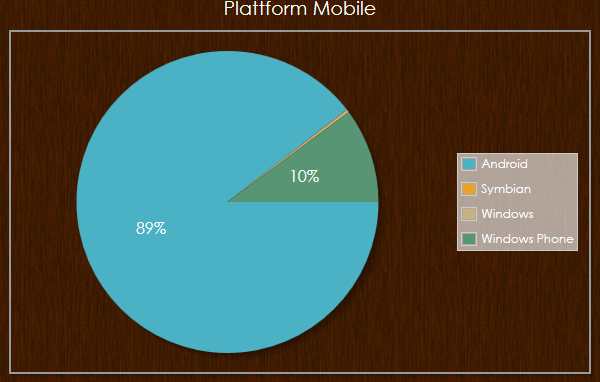
\includegraphics[keepaspectratio=true, width=8cm]{images/screenshots/statistics_os_Mob.png}
\caption{Browser PC}
\label{fig:instr_other_statistics_os_Mob}
\end{figure}
\subsubsection{Nutzer}
In dieser Statistik sind die Nutzer nach den Schulstufen und nach den Lehrern aufgeteilt. Hier kann herausgelesen werden welcher Jahrgang den Service am häufigsten nutzt. (siehe \autoref{fig:instr_other_statistics_user})
\begin{figure}[H]
\centering
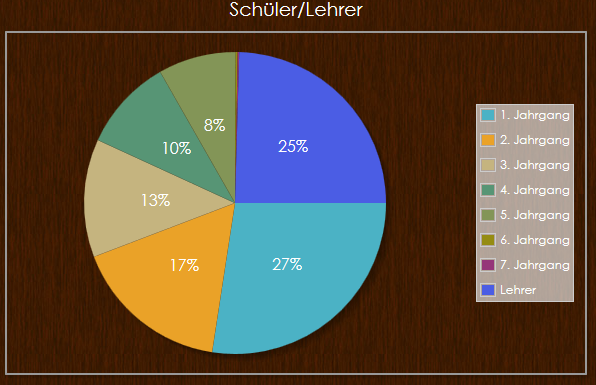
\includegraphics[keepaspectratio=true, width=8cm]{images/screenshots/statistics_user.png}
\caption{Nutzer}
\label{fig:instr_other_statistics_user}
\end{figure}
\subsubsection{Abteilungen}
In dieser Statistik werden die Nutzer nach ihrer Abteilung aufgeteilt, dabei werden nur die Schüler gezählt. Hier kann herausgelesen werden welche Abteilung den Service am häufigsten nutzt. (siehe \autoref{fig:instr_other_statistics_sections})
\begin{figure}[H]
\centering
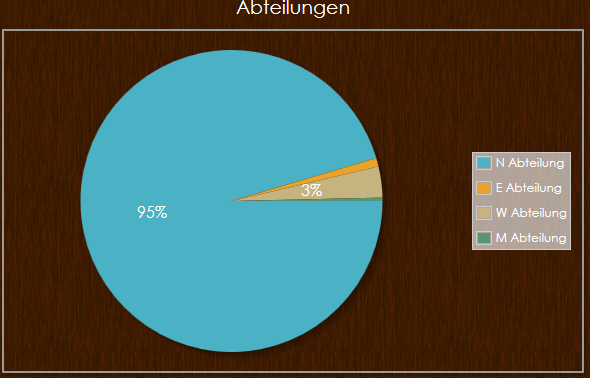
\includegraphics[keepaspectratio=true, width=8cm]{images/screenshots/statistics_sections.png}
\caption{Abteilungen}
\label{fig:instr_other_statistics_sections}
\end{figure}
\subsubsection{Supplierunen}
In dieser Statistik wird dargestellt welche Seite die User am häufigsten benützen, um die Supplierungen anzusehen. Dabei wird der Supplierplan im Web, Supplierplan in der App , der modifizierte Stundenplan in der App und der modifizierte Stundenplan im Web analysiert. (siehe \autoref{fig:instr_other_statistics_substitudes})
\begin{figure}[H]
\centering
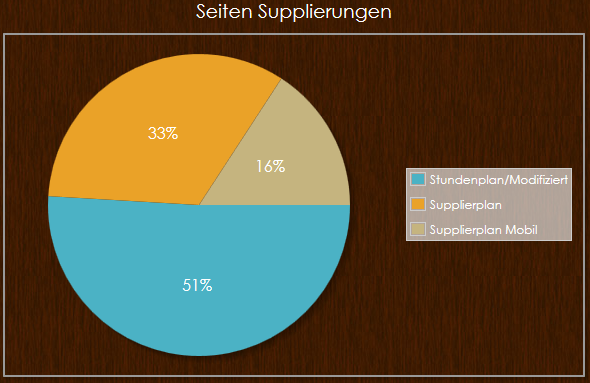
\includegraphics[keepaspectratio=true, width=8cm]{images/screenshots/statistics_substitudes.png}
\caption{Supplierungen}
\label{fig:instr_other_statistics_substitudes}
\end{figure}
\subsubsection{App/Web}
In dieser Statistik wird die App und die Webseite gegenübergestellt und man kann auslesen welcher Dienst öfters genutzt wird. (siehe \autoref{fig:instr_other_statistics_app_web})
\begin{figure}[H]
\centering
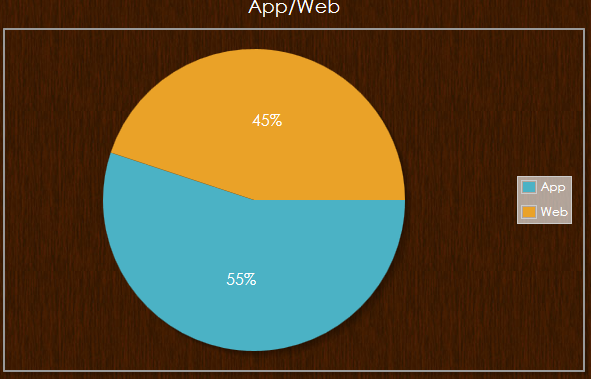
\includegraphics[keepaspectratio=true, width=8cm]{images/screenshots/statistics_app_web.png}
\caption{App/Web}
\label{fig:instr_other_statistics_app_web}
\end{figure}
\subsubsection{Seiten Web}
In dieser Statistik wird dargestellt welche Seiten die User auf der Webseite am häufigsten besuchen. (siehe \autoref{fig:instr_other_statistics_sites_web})
\begin{figure}[H]
\centering
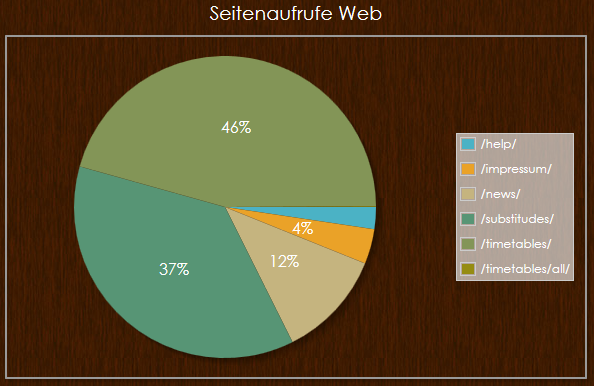
\includegraphics[keepaspectratio=true, width=8cm]{images/screenshots/statistics_sites_web.png}
\caption{Seiten Web}
\label{fig:instr_other_statistics_sites_web}
\end{figure}
\subsubsection{Seiten App}
In dieser Statistik wird dargestellt welche Seiten die User in der App am häufigsten besuchen. (siehe \autoref{fig:instr_other_statistics_sites_app})
\begin{figure}[H]
\centering
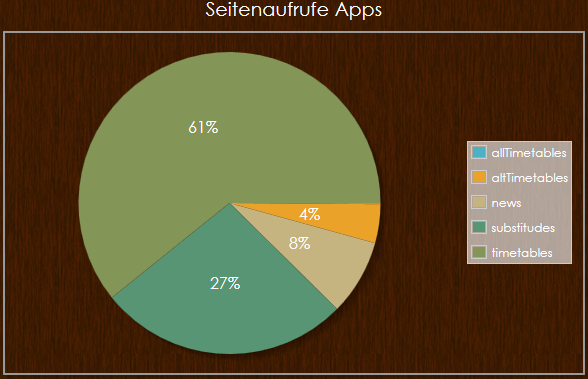
\includegraphics[keepaspectratio=true, width=8cm]{images/screenshots/statistics_sites_app.png}
\caption{Seiten App}
\label{fig:instr_other_statistics_sites_app}
\end{figure}
\subsubsection{Seitenaufrufe Stunden}
In dieser Statistik wird dargestellt, wie viele Seitenaufrufe im Durchschnitt in welcher Stunde am Tag auftreten. (siehe \autoref{fig:instr_other_statistics_view_day})
\begin{figure}[H]
\centering
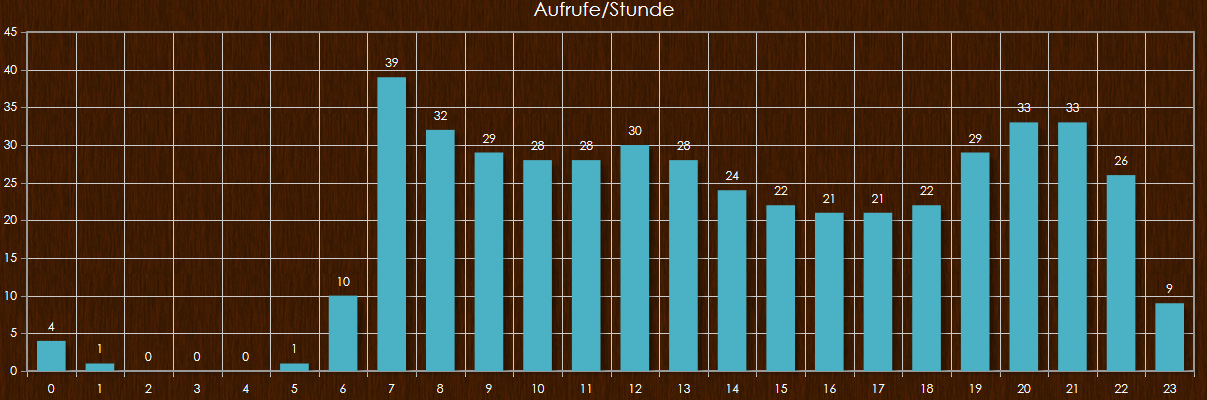
\includegraphics[keepaspectratio=true, width=17cm]{images/screenshots/statistics_views_hour.png}
\caption{Seitenaufrufe Stunden}
\label{fig:instr_other_statistics_view_day}
\end{figure}
\subsubsection{Seitenaufrufe täglich}
In dieser Statistik wird dargestellt, wie viele Seitenaufrufe jeden Tag verursacht werden. (siehe \autoref{fig:instr_other_statistics_views_day}) Hier kann auch, um bei vielen Tagen sich einen Überblick zu beschaffen, hineingezoomt werden. Dies macht man in dem man mit der linken Maustaste ein gewünschtes Fenster aufzieht. Heraus zoomen kann mit einem doppelten rechts Klick gemacht werden. (siehe \autoref{fig:instr_other_statistics_views_day_zoom})
\begin{figure}[H]
\centering
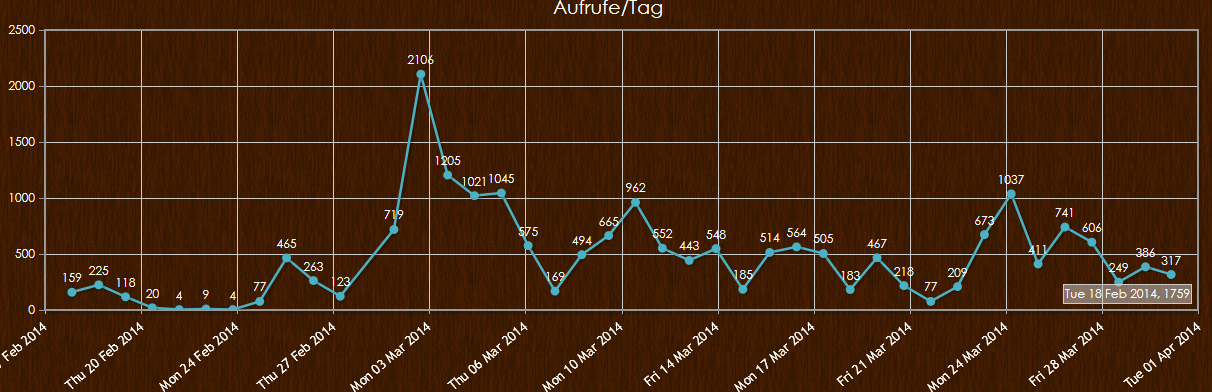
\includegraphics[keepaspectratio=true, width=17cm]{images/screenshots/statistics_views_day.png}
\caption{Seitenaufrufe täglich}
\label{fig:instr_other_statistics_views_day}
\end{figure}
\begin{figure}[H]
\centering
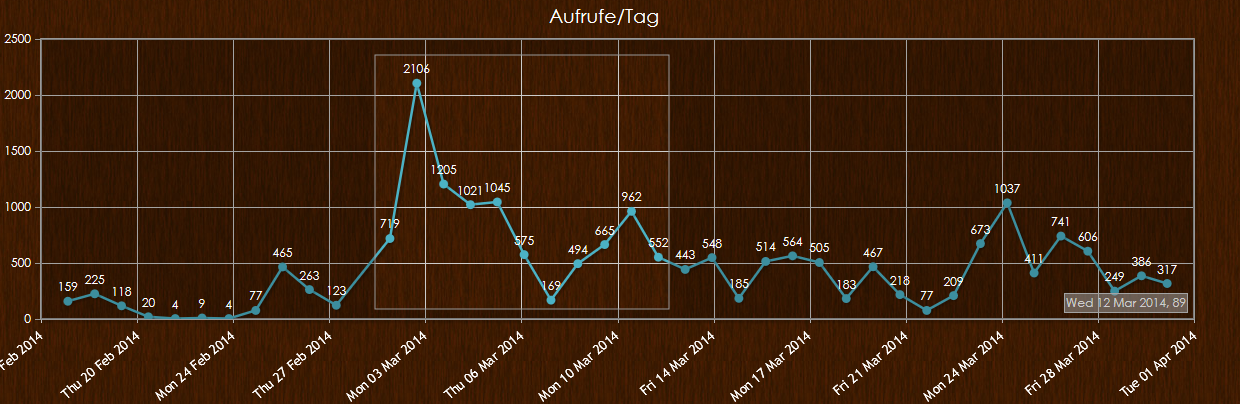
\includegraphics[keepaspectratio=true, width=17cm]{images/screenshots/statistics_views_day_zoom.png}
\caption{Seitenaufrufe täglich zoomen}
\label{fig:instr_other_statistics_views_day_zoom}
\end{figure}
\subsection{Räume}
Über diese Eingabemaske werden Räume bearbeitet und hinzugefügt (siehe \autoref{fig:instr_other_room_input}). Aus Gründen der Datenkonsistenz der Stunden- und Supplierpläne ist das Löschen von Räumen nicht möglich.
\begin{table}[H]
\centering
\begin{tabular}{p{3 cm}p{10 cm}}
   \toprule
   \textbf{Eingabefeld} & \textbf{Typ} \\
   \midrule
          \textbf{Name} & Textfeld - Pflichtfeld \newline Name des Raumes \\
          \hline
          Zuständiger Lehrer & Listenfeld - optional \newline Verantwortlicher Lehrer für den Raum\\
   \bottomrule
\end{tabular}
\caption{Eingabefelder Räume}
\end{table}
Änderungen und Ergänzungen sind über die Schaltfläche Übernehmen in den Eingabezeilen zu bestätigen.
\begin{figure}[H]
\centering
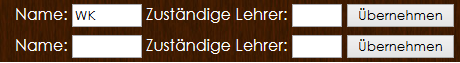
\includegraphics[keepaspectratio=true, width=10cm]{images/screenshots/rooms_input.png}
\caption{Eingabemaske Räume}
\label{fig:instr_other_room_input}
\end{figure}
\subsection{Klassen}
Über diese Eingabemaske werden Klassen bearbeitet und hinzugefügt (siehe \autoref{fig:instr_other_classes_input}). Aus Gründen der Datenkonsistenz der Stunden- und Supplierpläne ist das Löschen von Klassen nicht möglich. Jedoch können Klassen als unsichtbar gekennzeichnet werden (siehe \autoref{sec:instr_other_hidden}).
\begin{table}[H]
\centering
\begin{tabular}{p{3 cm}p{10 cm}}
   \toprule
   \textbf{Eingabefeld} & \textbf{Typ} \\
   \midrule
          \textbf{Name} & Textfeld - Pflichtfeld \newline Name der Klasse \\
          \hline
          \textbf{Abteilung} & Listenfeld - Pflichtfeld \\
          \hline
          Klassenvorstand & Listenfeld - optional \\
          \hline
          Stammklasse & Textfeld - optional \newline Zugeordneter Klassenraum \\
          \hline
          Unsichtbar & Checkbox \\
   \bottomrule
\end{tabular}
\caption{Eingabe Klassen}
\end{table}
Wanderklassen kann der Raum WK als Scheinklassenraum zugewiesen werden. Wird die Checkbox Unsichtbar bei einer Klasse gesetzt, wird diese in den Listenfelder nicht mehr angezeigt.\\
Änderungen und Ergänzungen sind über die Schaltfläche Übernehmen in den Eingabezeilen zu bestätigen.
\begin{figure}[H]
\centering

\includegraphics[keepaspectratio=true, width=17cm]{images/screenshots/classes_input.png}
\caption{Eingabemaske Klassen}
\label{fig:instr_other_classes_input}
\end{figure}
\subsection{Abteilungen}
Über diese Eingabemaske werden Abteilungen bearbeitet und hinzugefügt (siehe \autoref{fig:instr_other_sections_input}). Aus Gründen der Datenkonsistenz der Stunden- und Supplierpläne ist das Löschen von Abteilungen nicht möglich.
\begin{table}[H]
\centering
\begin{tabular}{p{3 cm}p{10 cm}}
   \toprule
   \textbf{Eingabefeld} & \textbf{Typ} \\
   \midrule
          \textbf{Name} & Textfeld - Pflichtfeld \newline Vollständiger Bezeichnung der Abteilung \\
          \hline
          \textbf{Kürzel} & Listenfeld - Pflichtfeld \\
          \hline
          \textbf{Abteilungsleiter} & Listenfeld - Pflichtfeld \\
   \bottomrule
\end{tabular}
\caption{Eingabe Abteilungen}
\end{table}
\begin{figure}[H]
\centering
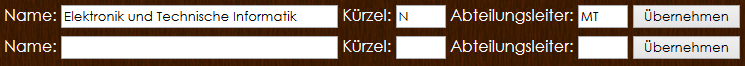
\includegraphics[keepaspectratio=true, width=17cm]{images/screenshots/sections_input.png}
\caption{Eingabemaske Abteilungen}
\label{fig:instr_other_sections_input}
\end{figure}
\subsection{Unsichtbar}\label{sec:instr_other_hidden}
Aus Sicherheitsgründen und Gründen der Datenkonsistenz dürfen manche Daten nicht gelöscht werden. Das Löschen ist nur dort möglich, wo explizit eine Checkbox Löschen vorhanden ist.\\
Um dennoch unnötige Einträge in den Listenfeldern zu vermeiden, können über die Checkbox Unsichtbar Einträge deaktiviert werden. Über die gleiche Funktion können diese Einträge dann wenn notwendig wieder aktiviert werden.
\subsection{DropDown-Menüs}
In zahlreichen Eingabefeldern sind Listen der zulässigen Eingaben hinterlegt, welche bei Beginn der Eingabe angezeigt werden. In Abhängigkeit der eingegebenen Zeichen wird die angezeigte Liste eingeschränkt. Ist die angezeigte Liste leer, so wurde kein übereinstimmender Eintrag gefunden und liegt wahrscheinlich eine Fehleingabe vor.

\end{document}